\chapter{MATRICES}\label{chap:matrices}

Las matrices son herramientas fundamentales en el álgebra lineal, con aplicaciones que abarcan desde la solución de sistemas de ecuaciones lineales hasta la representación de transformaciones lineales y la modelación de fenómenos en disciplinas como la física, la ingeniería y la economía. Para simplificar, en gran parte de este libro restringiremos nuestra atención al análisis de las matrices cuyas entradas son números reales. Sin embargo, también se estudiarán las matrices con entradas complejas, mismas que tienen gran importancia en muchas aplicaciones.

Este capítulo está dedicado al estudio de las matrices reales, sus propiedades algebraicas y las operaciones que pueden realizarse sobre ellas. Iniciaremos estableciendo el concepto de matriz real como una estructura rectangular formada por elementos del conjunto de los números reales. Posteriormente, introduciremos las operaciones básicas que se pueden realizar entre matrices: la suma, el producto por un escalar y el producto matricial, analizando las condiciones necesarias para que estas operaciones estén bien definidas y sus propiedades fundamentales, como la asociatividad, distributividad y conmutatividad.

Las matrices reales son más que simples arreglos de números; representan sistemas lineales y sirven como base para conceptos avanzados, como determinantes, transformaciones lineales y espacios vectoriales. En este capítulo, también exploraremos tipos específicos de matrices reales, como las matrices cuadradas, diagonales, simétricas y triangulares, cada una con propiedades particulares que las hacen esenciales en aplicaciones matemáticas y computacionales.

El estudio de las matrices reales no solo proporciona herramientas algebraicas para manipular datos y resolver problemas matemáticos, sino que también abre la puerta a la comprensión de conceptos más abstractos, como valores y vectores propios, y su conexión con la diagonalización. Este enfoque nos permitirá sentar las bases para abordar temas más avanzados en capítulos posteriores, donde se extiende el análisis a matrices con entradas complejas y espacios vectoriales complejos.

\newpage

\section{El espacio vectorial de matrices}

\begin{definicion}{}{}
    Una \emph{matriz} de $m \times n$ es un arreglo rectangular de $mn$ números reales ordenados en $m$ filas (renglones) horizontales y $n$ columnas verticales:
    $$\makecell{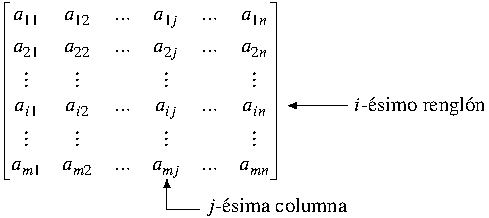
\includegraphics[page=1]{Externalizacion/C2/MatricesC2.pdf}}$$
    Nos referimos al número $a_{ij}$, que está en la $i$-ésima fila (renglón) y la $j$-ésima columna donde $i \in \left\{ 1, 2, \dots, m \right\}$ y $j \in \left\{ 1, 2, \dots, n \right\}$, como el $ij$-ésimo \emph{elemento} de dicha matriz, o la \emph{entrada} $(i, j)$ de dicha matriz.
\end{definicion}

Vamos a denotar a las matrices con letras mayúsculas: $A$, $B$, $C$, $D$, $\dots$, y al arreglo de la matriz $A$, lo denotaremos por $[ a_{ij} ]$. Diremos que $A$ es $m$ por $n$ (que se escribe $m \times n$). Al conjunto de las matrices de tamaño $m \times n$ con entradas en $\RR$ lo denotaremos por $\matrizmn$, donde
$$\matrizmn = \left\{ [ a_{ij} ] \mid a_{ij} \in \RR, \text{ con } i \in \{ 1, 2, \dots, m \} \text{ ~y~ } j \in \{ 1, 2, \dots, n \} \right\}.$$
Si $m = n$, decimos que $A$ es una \emph{matriz cuadrada de orden $n$}, y que los números $a_{11}, a_{22}, \dots, a_{nn}$ forman la \emph{diagonal principal de $A$}.

\begin{examplebox}{}{}
    Sean
    \begin{matrizn}
        \makecell{\includegraphics[page=2]{Externalizacion/C2/MatricesC2.pdf}}
    \end{matrizn}
    Entonces $A$ es una matriz de tamaño $2 \times 3$ con $a_{12} = 0$, $a_{13} = 3$, $a_{22} = 1$, $a_{23} = 8$; $B$ es una matriz de tamaño $2 \times 2$ con $b_{11} = 1$, $b_{22} = -3$; $C$ es una matriz de tamaño $3 \times 1$ con $c_{11} = 1$, $c_{21} = -1$, $c_{31} = 2$.
\end{examplebox}

\begin{definicion}{}{operacionesMatriz}
    Dadas $A$, $B \in \matrizmn$ con $A = [ a_{ij} ]$, $B = [ b_{ij} ]$, y además, $\alpha \in \RR$, definimos la matriz suma de $A$ y $B$ (denotada por $A + B$) y la matriz producto por escalar de $\alpha$ y $A$ (denotada por $\alpha \cdot A$), respectivamente como
    \begin{alignat*}{2}
        + & : & \qquad \matrizmn \times \matrizmn & \longrightarrow \matrizmn \\
        & & (A, B) & \longmapsto A + B \\
        & \\
        \cdot & : & \qquad \RR \times \matrizmn & \longrightarrow \matrizmn \\
        & & (\alpha, A) & \longmapsto \alpha \cdot A
    \end{alignat*}
    Es decir, para toda $i \in \left\{ 1, 2, \dots, m \right\}$ y $j \in \left\{ 1, 2, \dots, n \right\}$ tenemos que
    $$[ a_{ij} ] + [ b_{ij} ] = [ a_{ij} + b_{ij} ], \quad \alpha \cdot [ a_{ij} ] = [ \alpha \cdot a_{ij} ].$$
\end{definicion}

\begin{examplebox}{}{}
    Sean
    $$A = \begin{bmatrix*}[r]
        1 & -2 & 4 \\
        2 & -1 & 3
    \end{bmatrix*} \quad \text{ y } \quad B = \begin{bmatrix*}[r]
        0 & 2 & -4 \\
        1 & 3 & -1
    \end{bmatrix*}.$$
    Entonces
    $$A + B = \begin{bmatrix}
        1 + 0 & -2 + 2 & 4 + (-4) \\
        2 + 1 & -1 + 3 & 3 + (-1)
    \end{bmatrix} = \begin{bmatrix}
        1 & 0 & 0 \\
        3 & 2 & 2
    \end{bmatrix}.$$
\end{examplebox}

\newpage

\begin{definicion}{}{}
    Decimos que dos matrices $A$ y $B$ son iguales si:
    \begin{enumerate}[label=\roman*), topsep=6pt, itemsep=0pt]
        \item Tienen el mismo tamaño.
        \item Tienen las mismas entradas.
    \end{enumerate}
\end{definicion}

\begin{theorem}{}{}
    El conjunto de las matrices de tamaño $m \times n$ con entradas en $\RR$
    $$\matrizmn = \left\{ [ a_{ij} ] \mid a_{ij} \in \RR, \text{ con } i \in \{ 1, 2, \dots, m \} \text{ ~y~ } j \in \{ 1, 2, \dots, n \} \right\}$$
    con las operaciones de la definición \ref{definicion:operacionesMatriz}, es un espacio vectorial sobre $\RR$.

    \tcblower
    \demostracion Probemos que el conjunto $\matrizmn$ cumple las diez propiedades de la definición \ref{definicion:espvec} como sigue:
    \begin{enumerate}[label=\roman*), topsep=6pt, itemsep=0pt]
        \item Es claro que se cumple la primer propiedad de suma, pues dados $[ a_{ij} ]$, $[ b_{ij} ] \in \matrizmn$
        \begin{align*}
            [ a_{ij} ] + [ b_{ij} ] & = [ a_{ij} +b_{ij} ] \in \matrizmn && \text{por def. de suma de matrices}
        \end{align*}
        \item Se deja como ejercicio al lector.
        \item Dados $[ a_{ij} ]$, $[ b_{ij} ] \in \matrizmn$
        \begin{align*}
            [ a_{ij} ] + [ b_{ij} ] & = [ a_{ij} +b_{ij} ] && \text{por def. de suma de matrices} \\
            & = [ b_{ij} + a_{ij} ] && \text{por conmutatividad en $\RR$} \\
            & = [ b_{ij} ] + [ a_{ij} ]
        \end{align*}
        Por tanto, se cumple la conmutatividad.
        \item Existe $[ 0_{ij} ] \in \matrizmn$, siendo
        \begin{matrizn}
            \makecell{\includegraphics[page=3]{Externalizacion/C2/MatricesC2.pdf}}
        \end{matrizn}
        tal que
        \begin{align*}
            [ a_{ij} ] + [ 0_{ij} ] & = [ a_{ij} + 0 ] && \text{por def. de suma de matrices} \\
            & = [ a_{ij} ] && \text{por neutro aditivo en $\RR$}
        \end{align*}
        Por tanto, se cumple la propiedad del neutro aditivo.
        \item Dada $[ a_{ij} ] \in \matrizmn$, existe $[ - a_{ij} ] \in \matrizmn$ tal que
        \begin{align*}
            [ a_{ij} ] + [ - a_{ij} ] & = [ a_{ij} -a_{ij} ] && \text{por def. de suma de matrices} \\
            & = [ 0_{ij} ] && \text{por inverso aditivo en $\RR$}
        \end{align*}
        A la matriz $[ -a_{ij} ]$ se le llama matriz inversa de $[ a_{ij} ]$ para la suma. Por tanto, se cumple la propiedad del inverso aditivo.
        \item Es claro que se cumple la primer propiedad de multiplicación escalar, pues dados $\alpha \in \RR$ y $[ a_{ij} ] \in \matrizmn$
        \begin{align*}
            \alpha \cdot [ a_{ij} ] & = [ \alpha \cdot a_{ij} ] \in \matrizmn && \text{por def. de multiplicación escalar}
        \end{align*}
        \item Dados $\alpha$, $\beta \in \RR$ y $[ a_{ij} ] \in \matrizmn$
        \begin{align*}
            \alpha \cdot \big( \beta \cdot [ a_{ij} ] \big) & = \alpha \cdot [ \beta \cdot a_{ij} ] && \text{por def. de multiplicación escalar} \\
            & = [ \alpha \cdot ( \beta \cdot a_{ij}) ] && \text{por def. de multiplicación escalar} \\
            & = [ (\alpha \cdot \beta) \cdot a_{ij} ] && \text{por conmitatividad en $\RR$} \\
            & = ( \alpha \cdot \beta ) \cdot [ a_{ij} ]
        \end{align*}
        Por tanto, se cumple la asociatividad.
        \item Se deja como ejercicio al lector.
        \item Se deja como ejercicio al lector.
        \item Se deja como ejercicio al lector.
    \end{enumerate}
    Por tanto, $\matrizmn$ es un espacio vectorial sobre $\RR$.
\end{theorem}

\section{Multiplicación de matrices y propiedades}

\begin{definicion}{}{JUNSJSNSN}
    Sean $\mathbb{u}$, $\mathbb{v} \in \RR[n]$ con
    \begin{matrizn}
        \makecell{\includegraphics[page=4]{Externalizacion/C2/MatricesC2.pdf}}
    \end{matrizn}
    Se define el \emph{producto punto} o \emph{producto escalar} de los vectores $\mathbb{u}$ y $\mathbb{v}$, denotado por $\mathbb{u} \bullet \mathbb{v}$, como sigue:
    $$\mathbb{u} \bullet \mathbb{v} = u_1v_1 + u_2v_2 + \cdots + u_nv_n = \sum_{i=1}^{n} u_iv_i.$$
\end{definicion}

\begin{theorem}{}{propiedadespunto1}
    El producto punto cumple lo siguiente:
    \begin{enumerate}[label=\roman*), topsep=6pt, itemsep=0pt]
        \item $\mathbb{u} \bullet \mathbb{0} = 0$, siendo $\mathbb{u}$, $\mathbb{0} \in \RR[n]$ y $0 \in \RR$.
        \item $\mathbb{u} \bullet \mathbb{v} = \mathbb{v} \bullet \mathbb{u}$, siendo $\mathbb{u}$, $\mathbb{v} \in \RR[n]$.
        \item $\mathbb{u} \bullet (\mathbb{v} + \mathbb{w}) = \mathbb{u} \bullet \mathbb{v} + \mathbb{u} \bullet \mathbb{w}$, siendo $\mathbb{u}$, $\mathbb{v}$, $\mathbb{w} \in \RR[n]$.
        \item $(\alpha \cdot \mathbb{u}) \bullet \mathbb{v} = \mathbb{u} \bullet (\alpha \cdot \mathbb{v}) = \alpha \cdot (\mathbb{u} \bullet \mathbb{v})$, siendo $\mathbb{u}$, $\mathbb{v} \in \RR[n]$ y $\alpha \in \RR$.
    \end{enumerate}

    \tcblower
    \demostracion
    \begin{enumerate}[label=\roman*), topsep=6pt, itemsep=0pt]
        \item Sea $\mathbb{u}$, $\mathbb{0} \in \RR[n]$,
        \begin{matrizn}
            \makecell{\includegraphics[page=5]{Externalizacion/C2/MatricesC2.pdf}}
        \end{matrizn}
        \item Sea $\mathbb{u}$, $\mathbb{v} \in \RR[n]$,
        \begin{matrizn}
            \makecell{\includegraphics[page=6]{Externalizacion/C2/MatricesC2.pdf}}
        \end{matrizn}
        \item Sea $\mathbb{u}$, $\mathbb{v}$, $\mathbb{w} \in \RR[n]$,
        \begin{matrizn}
            \makecell{\includegraphics[page=7]{Externalizacion/C2/MatricesC2.pdf}}
        \end{matrizn}
        \item Sea $\mathbb{u}$, $\mathbb{v} \in \RR[n]$, $\alpha \in \RR$,
        \begin{matrizn}
            \makecell{\includegraphics[page=8]{Externalizacion/C2/MatricesC2.pdf}}
        \end{matrizn}
    \end{enumerate}
\end{theorem}

\begin{examplebox}{}{}
    Consideremos dos vectores en $\RR[3]$
    $$\makecell{\includegraphics[page=9]{Externalizacion/C2/MatricesC2.pdf}}$$
    El producto punto de estos dos vectores se calcula como:
    $$\mathbb{u} \bullet \mathbb{v} = (2)(4) + (-3)(5) + (1)(-2) = 8 - 15 - 2 = -9$$
    Por lo tanto, el producto punto de $\mathbb{u}$ y $\mathbb{v}$ es $-9$.
\end{examplebox}

Las matrices son una forma elegante y eficiente de organizar y manipular conjuntos de números. Son especialmente útiles en el álgebra lineal, ya que nos permiten representar sistemas de ecuaciones lineales, realizar transformaciones lineales, modelar datos y mucho más.
    
El producto de matrices es una operación crucial que nos permite combinar dos matrices para obtener una nueva matriz. Pero a diferencia de la suma o resta de matrices, el producto no es simplemente una operación elemento por elemento. En cambio, implica un procedimiento más complejo que puede parecer un poco misterioso al principio. Supongamos que tenemos dos matrices, $A$ y $B$. Para multiplicar $A$ por $B$ (denotado como $AB$), tomamos cada fila de $A$ y la “emparejamos” con cada columna de $B$, realizando una serie de multiplicaciones y sumas. Es importante tener en cuenta que no siempre se pueden multiplicar matrices.

\newpage
    
Para que sea más claro de ver, observe la figura \ref{bhfrfbhfbhh}. Proporcionaremos ejemplos prácticos y una variedad de ejercicios para que los lectores puedan poner en práctica sus conocimientos sobre el producto de matrices.
\begin{figure}[h!]
    \centering
    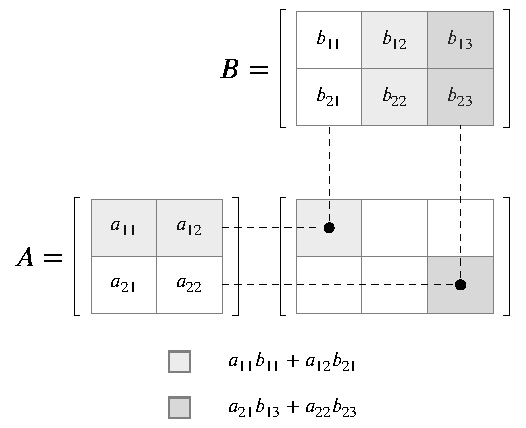
\includegraphics[scale=0.87]{Images/Capitulo2/ProdMatrices.pdf}
    \caption{La representación del producto de matrices}\label{bhfrfbhfbhh}
\end{figure}

\begin{examplebox}{}{}
    Sean las matrices $A \in \mathcalm{M}_{2 \times 3}(\RR)$ y $B \in \mathcalm{M}_{3 \times 4}(\RR)$ dadas por
    \begin{matrizn}
        \makecell{\includegraphics[page=10]{Externalizacion/C2/MatricesC2.pdf}}
    \end{matrizn}
    Al multiplicar la matriz $A$ por la matriz $B$ como la figura \ref{bhfrfbhfbhh}, obtenemos:
    \begin{matrizn}
        \makecell{\includegraphics[page=11]{Externalizacion/C2/MatricesC2.pdf}}
    \end{matrizn}
\end{examplebox}

\begin{definicion}{}{matrixprod}
    Sean $A = [ a_{ij} ] \in \mathcalm{M}_{m \times p}(\RR)$ y $B = [ b_{jk} ] \in \mathcalm{M}_{p \times n}(\RR)$. Se define el producto de las matrices $A$ con $B$, como sigue
    \begin{matrizn}
        \makecell{\includegraphics[page=12]{Externalizacion/C2/MatricesC2.pdf}}
    \end{matrizn}
    donde
    \begin{equation}
        c_{ik} = \sum_{q=1}^{p} a_{iq}b_{qk} = a_{i1}b_{1k} + a_{i2}b_{2k} + \cdots + a_{ip}b_{pk} \label{eqcusjahha}
    \end{equation}
\end{definicion}

\newpage

Nótese que no siempre se puede multiplicar matrices. Dos matrices se pueden multiplicar únicamente si el número de columnas de la primera matriz es igual al número de renglones de la segunda. De otro modo, los vectores que forman el renglón $i$ en $A$ y la columna $j$ de $B$ no tendrán el mismo número de componentes y el producto punto en la ecuación \eqref{eqcusjahha} no estará definido. Dicho de otro modo, las matrices $A$ y $B$ serán \textit{incompatibles} bajo la multiplicación.
\sideTable[\label{tab:1}]{
    \centering
    \vspace{3cm}\begin{tabular}{ll}
        \toprule
        \textbf{Grupo} & \textbf{Elementos} \\
        \midrule
        $X$ & $a_1$, $a_2$, $a_3$, $a_4$ \\
        $Y$ & $b_1$, $b_2$, $b_3$, $b_4$, $b_5$, $b_6$ \\
        $Z$ & $c_1$, $c_2$, $c_3$, $c_4$, $c_5$ \\
        \bottomrule
    \end{tabular}
}
\begin{examplebox}{}{enfermedadescone}
    En este ejemplo se muestra la forma en la cual se puede usar la multiplicación de matrices para modelar la manera en que se extiende una enfermedad contagiosa. Las enfermedades contagiosas son aquellas que se propagan de una persona a otra a través del contacto directo. Los ejemplos incluyen la gripe, el resfriado común y la COVID-19. Considere tres grupos de personas $X$, $Y$ y $Z$ con $4$, $6$ y $5$ elementos respectivamente como se muestra en la tabla \ref{tab:1}. Suponga que cuatro individuos han contraído esta enfermedad. Este grupo entra en contacto con seis personas de un segundo grupo. Estos contactos, llamados \textit{contactos directos}, se pueden representar por una matriz de $4 \times 6$. Consideremos la siguiente matriz para los grupos $X$ y $Y$:
    $$\makecell{\includegraphics[page=13]{Externalizacion/C2/MatricesC2.pdf}}$$
    En este caso se hace $a_{ij} = 1$ si la $i$-ésima persona del primer grupo entra en contacto con la $j$-ésima persona del segundo grupo. Por ejemplo, el $1$ en la posición $(2, 4)$ significa que la segunda persona del primer grupo (infectada) entró en contacto con la cuarta persona del segundo grupo. Ahora suponga que un tercer grupo de cinco personas tiene varios contactos directos con individuos del segundo grupo. Esto también se puede representar mediante una matriz.
    \begin{matrizn}
        \makecell{\includegraphics[page=14]{Externalizacion/C2/MatricesC2.pdf}}
    \end{matrizn}
    Observe que $b_{64} = 0$, lo que quiere decir que la sexta persona del segundo grupo no tiene contacto con la cuarta persona del tercer grupo. Los contactos \textit{indirectos} o de \textit{segundo orden} entre individuos del primero y tercer grupos se representan mediante la matriz de $4 \times 5$, $C = AB$. Para ver esto, observe que una persona del grupo $3$ puede quedar contagiada por alguien del grupo $2$, quien a su vez fue contagiada por alguien del grupo $1$. Por ejemplo, como $a_{24} = 1$ y $b_{45} = 1$ se ve que, indirectamente, la quinta persona del grupo $3$ tuvo contacto (a través de la cuarta persona del grupo $2$) con la segunda persona del grupo $1$. El número total de contactos indirectos entre la segunda persona del grupo $1$ y la quinta persona del grupo $3$ está dado por
    \begin{align*}
        c_{25} & = a_{21}b_{15} + a_{22}b_{25} + a_{23}b_{35} + a_{24}b_{45} + a_{25}b_{55} + a_{26}b_{65} \\
        & = 1 \cdot 1 + 0 \cdot 0 + 0 \cdot 0 + 1 \cdot 1 + 0 \cdot 0 + 1 \cdot 0 = 2
    \end{align*}
    Así pues,
    \begin{matrizn}
        \makecell{\includegraphics[page=15]{Externalizacion/C2/MatricesC2.pdf}}
    \end{matrizn}
    Observe que únicamente la segunda persona del grupo $3$ no tiene contactos indirectos con la enfermedad. La quinta persona de este grupo tiene $2 + 1 + 1 = 4$ contactos de segundo orden.
\end{examplebox}

\newpage

\begin{examplebox}{}{}
    Un torneo de Tenis se puede organizar de la siguiente manera. Cada uno de los $n$ tenistas juega contra todas los demás y se registran los resultados en una matriz $R = [ r_{ij} ] \in \mathcalm{M}_{n \times n}(\RR)$ como sigue:
    $$r_{ij} = \begin{cases}
        1, & \text{ si el jugador $i$ le gana al $j$} \\
        0, & \text{ si el jugador $i$ pierde contra el $j$} \\
        0, & \text{ si $i = j$}
    \end{cases}$$
    Se asigna al tenista $i$ la calificación siguiente:
    \begin{equation}
        S_i = \sum_{j=1}^{n} r_{ij} + \frac{1}{2} \sum_{j=1}^{n} \left( R^{2} \right)_{ij} \label{ec28}
    \end{equation}
    Para un torneo de $n = 4$ tenistas, tenemos
    \begin{matrizn}
        \makecell{\includegraphics[page=16]{Externalizacion/C2/MatricesC2.pdf}}
    \end{matrizn}
    Para clasificar a los jugadores, primero calculemos $R^{2}$ como sigue:
    \begin{matrizn}
        \makecell{\includegraphics[page=17]{Externalizacion/C2/MatricesC2.pdf}}
    \end{matrizn}
    Así, utilizando la ecuación \eqref{ec28}, obtenemos:
    \begin{align*}
        S_1 & = 1 + \frac{1}{2} (2) & S_2 & = 2 + \frac{1}{2} (3) & S_3 & = 1 + \frac{1}{2} (1) & S_4 & = 2 + \frac{1}{2} (2) \\
        & = 2 & & = \frac{7}{2} & & = \frac{3}{2} & & = 3
    \end{align*}
    Por tanto, $S_1 = 2$, $S_2 = 3.5$, $S_3 = 1.5$ y $S_4 = 3$, y además
    $$S_3 < S_1 < S_4 < S_2.$$
    El puntaje es el número de juegos ganados por el jugador $i$ más la mitad del número de juegos ganados por los jugadores a quienes el jugador $i$ venció.
\end{examplebox}

\begin{examplebox}{}{}
    En inteligencia artificial, el producto de matrices es esencial para calcular la salida de una capa en una \emph{red neuronal artificial}. Supongamos que tenemos una \emph{capa neuronal} con 3 neuronas y 4 entradas, donde: $X$ es contiene todas las características del dato, $W$ es la \emph{matriz de pesos} que conecta las entradas con las neuronas, $B$ contiene todos los \emph{sesgos} de los datos, $Y$ es la \emph{salida de la capa neuronal}. Así,
    \begin{matrizn}
        \makecell{\includegraphics[page=18]{Externalizacion/C2/MatricesC2.pdf}}
    \end{matrizn}
    La salida de la capa se obtiene mediante el producto de matrices:
    $$Y = W X + B$$
    Expandiendo este cálculo, el cual se realiza en \emph{todas las capas de una red neuronal}:
    $$\makecell{\includegraphics[page=19]{Externalizacion/C2/MatricesC2.pdf}}$$
\end{examplebox}

\newpage

\begin{theorem}{}{}
    El producto de matrices es asociativo.
\end{theorem}

El producto de matrices, a diferencia de la multiplicación numérica, no es conmutativo en general. Esto significa que el orden de los factores altera significativamente el resultado. Para ilustrar este fenómeno, consideremos el siguiente contraejemplo con matrices cuadradas de orden 2:
$$A = \begin{bmatrix}
    1 & 1 \\
    0 & 1
\end{bmatrix} \quad \text{ y } \quad B = \begin{bmatrix}
    2 & 1 \\
    1 & 1
\end{bmatrix}$$
Calculamos primero $AB$,
\begin{align*}
    AB & = \begin{bmatrix}
        1 & 1 \\
        0 & 1
    \end{bmatrix} \begin{bmatrix}
        2 & 1 \\
        1 & 1
    \end{bmatrix} \\
    & = \begin{bmatrix}
        3 & 2 \\
        1 & 1
    \end{bmatrix}
\end{align*}
Ahora, invirtiendo el orden
\begin{align*}
    BA & = \begin{bmatrix}
        2 & 1 \\
        1 & 1
    \end{bmatrix} \begin{bmatrix}
        1 & 1 \\
        0 & 1
    \end{bmatrix} \\
    & = \begin{bmatrix}
        2 & 3 \\
        1 & 2
    \end{bmatrix}
\end{align*}
Así que, en general $AB \neq BA$.

De aquí en adelante se escribirá el producto de tres matrices simplemente como $ABC$. Se puede hacer esto porque $(AB)C = A(BC)$; entonces se obtiene la misma respuesta independientemente de cómo se lleve a cabo la multiplicación (siempre y cuando no se conmute ninguna de las matrices). La ley asociativa se puede extender a productos de más matrices. Por ejemplo, suponga que $AB$, $BC$ y $CD$ están definidas. Entonces
$$ABCD = A\big(B(CD)\big) = \big((AB)C\big)D = A(BC)D = (AB)(CD)$$
Existe una ley distributiva para la multiplicación de matrices.

\begin{theorem}{}{}
    Si todas las sumas y todos los productos siguientes están definidos, entonces
    $$A(B + C) = AB + AC \quad \text{ y } \quad (A + B)C = AC + BC$$

    \tcblower
    \demostracion Demostraremos la primer igualdad, la segunda se deja como ejercicio al lector. Sean $A \in \mathcalm{M}_{m \times p}(\RR)$ con $A = [ a_{ij} ]$, y $B$, $C \in \mathcalm{M}_{p \times n}(\RR)$ con $B = [ b_{kj} ]$ y $C = [ c_{kj} ]$. Por las dimensiones de las matrices, la suma $B + C$ y los productos $AB$, $AC$ están bien definidos. Primero calculamos $B + C$, operación que se realiza entrada por entrada
    \begin{matrizn}
        \makecell{\includegraphics[page=20]{Externalizacion/C2/MatricesC2.pdf}}
    \end{matrizn}
    Aplicando la definición de multiplicación matricial, cada entrada $(i, j)$ del producto es el producto punto de la fila $i$ de $A$ con la columna $j$ de $B + C$,
    \begin{matrizn}
        \makecell{\includegraphics[page=21]{Externalizacion/C2/MatricesC2.pdf}}
    \end{matrizn}
    En cada entrada, la distributividad en $\RR$ permite separar las sumas
    $$\sum_{q=1}^{p} a_{iq}(b_{qj} + c_{qj}) = \sum_{q=1}^{p} a_{iq}b_{qj} + \sum_{q=1}^{p} a_{iq}c_{qj}$$
    Esto permite expresar la suma de dos productos matriciales, es decir,
    $$\makecell{\includegraphics[page=22]{Externalizacion/C2/MatricesC2.pdf}}$$
    Por lo tanto, queda demostrada la igualdad $A(B + C) = AB + AC$.
\end{theorem}

Cuando trabajamos con una misma matriz cuadrada, es posible definir potencias enteras positivas mediante la multiplicación iterada. Es decir, si $A \in \mathcalm{M}_{n \times n}(\RR)$ y $n \in \NN$, definimos $A^n$ como
$$A^n = \underbrace{A A \cdots A}_{n-\text{veces}}$$

A continuación, presentaremos una variedad de matrices con diferentes propiedades y características. Cada tipo de matriz posee atributos específicos que permiten clasificarla y estudiarla en el álgebra lineal.

\begin{definicion}{}{matriz-idempotente}
    Sea $A \in \mathcalm{M}_{n \times n}(\RR)$, decimos que $A$ es una matriz idempotente si $A^2 = A$.
\end{definicion}

\newpage

\begin{examplebox}{}{idempotentem}
    Sea $A =\begin{bNiceMatrix}[cell-space-limits=3pt,r]
        -1 & 3 & 5\vphantom{^A} \\
        1 & -3 & -5 \\
        -1 & 3 & 5\vphantom{_A} \\
    \end{bNiceMatrix}$, entonces
    \begin{matrizn}
        \makecell{\includegraphics[page=23]{Externalizacion/C2/MatricesC2.pdf}}
    \end{matrizn}
    Por tanto, $A$ es idempotente.
\end{examplebox}

\begin{definicion}{}{}
    Sea $A \in \mathcalm{M}_{n \times n}(\RR)$, decimos que $A$ es una matriz nilpotente si existe un entero positivo $p$ tal que $A^p = \mathbb{0}$. El grado o índice de nilpotencia es el menor entero positivo $p$ tal que $A^p = \mathbb{0}$.
\end{definicion}

\begin{examplebox}{}{}
    Sea $A = \begin{bmatrix*}[r]
        1 & 1 \\
        -1 & -1 \\
    \end{bmatrix*}$, entonces
    $$A^2 = \begin{bmatrix*}[r]
        1 & 1 \\
        -1 & -1 \\
    \end{bmatrix*} \begin{bmatrix*}[r]
        1 & 1 \\
        -1 & -1 \\
    \end{bmatrix*} = \begin{bmatrix*}[r]
        0 & 0 \\
        0 & 0 \\
    \end{bmatrix*}.$$
    Por tanto, $A$ es nilpotente de índice de nilpotencia 2.
\end{examplebox}

Una matriz que desempeña un papel central en el álgebra lineal es la llamada matriz identidad. Esta matriz actúa como el elemento neutro de la multiplicación matricial, análoga al número uno en la multiplicación de escalares.

\begin{definicion}{}{}
    La \emph{matriz identidad} $I_n$ es una matriz de $n \times n$ cuyos elementos de la diagonal principal son iguales a $1$ y todos los demás son $0$. Esto es,
    $$I_n = [ \delta_{ij} ] = \begin{cases}
        1 & \text{ si } i = j \\
        0 & \text{ si } i \neq j
    \end{cases}$$
\end{definicion}

Si no es importante enfatizar el tamaño, escribiremos solamente $I$ para denotar a la matriz identidad. Para explicar el papel de las matrices identidad en la aritmética de matrices, consideremos el efecto de multiplicar una matriz general $A$ de tamaño $2 \times 3$ en cada lado por una matriz identidad. Multiplicar por la derecha con la matriz identidad $3 \times 3$ da
\begin{matrizn}
    \makecell{\includegraphics[page=24]{Externalizacion/C2/MatricesC2.pdf}}
\end{matrizn}
y multiplicar por la izquierda con la matriz identidad $2 \times 2$ da
$$I_2 A = \begin{bmatrix}
    1 & 0 \\
    0 & 1
\end{bmatrix} \begin{bmatrix}
    a_{11} & a_{12} & a_{13} \\
    a_{21} & a_{22} & a_{23}
\end{bmatrix} = \begin{bmatrix}
    a_{11} & a_{12} & a_{13} \\
    a_{21} & a_{22} & a_{23}
\end{bmatrix} = A.$$
El mismo resultado se cumple en general; es decir, si $A$ es cualquier matriz $m \times n$,% entonces
$$A I_n = A \quad \text{ y } \quad I_m A = A.$$
Dado que las matrices pueden elevarse a potencias y combinarse mediante operaciones algebraicas, es natural extender a ellas la noción de aplicarles un polinomio.

\begin{definicion}{}{}
    Sea $A \in \mathcalm{M}_{n \times n} (\RR)$ y sea $f(x) \in P_m$, con
    $$f(x) = a_mx^m + \cdots + a_1x + a_0.$$
    Definimos a $f(A)$ como:
    $$f(A) = a_mA^m + \cdots + a_1A + a_0I_n.$$
\end{definicion}

\newpage

\begin{examplebox}{}{}
    Si $f(x) = x^2 -5x +2$ y $A = \begin{bmatrix}
        2 & 0 \\
        4 & 5 \\
    \end{bmatrix}$, entonces:
    $$f(A) = \begin{bmatrix}
        2 & 0 \\
        4 & 5 \\
    \end{bmatrix} \begin{bmatrix}
        2 & 0 \\
        4 & 5 \\
    \end{bmatrix} -5 \begin{bmatrix}
        2 & 0 \\
        4 & 5 \\
    \end{bmatrix} +2 \begin{bmatrix}
        1 & 0 \\
        0 & 1 \\
    \end{bmatrix} = \begin{bmatrix*}[r]
        -4 & 0 \\
        8 & 2 \\
    \end{bmatrix*}.$$
\end{examplebox}

\begin{definicion}{}{}
    Si $A$ es una matriz cuadrada, entonces la \textit{traza de $A$}, denotada por $\operatorname{Tr}(A)$, se define como la suma de las entradas en la diagonal principal de $A$. La traza de $A$ no está definida si $A$ no es una matriz cuadrada.
\end{definicion}

\begin{examplebox}{}{}
    Si consideramos la matriz del ejemplo \ref{examplebox:idempotentem}, entonces la traza de $A$ es
    $$\operatorname{Tr}(A) = (-1) + (-3) + 5 = 1.$$
\end{examplebox}

\begin{definicion}{}{transpuestaijji}
    Sea $A \in \mathcalm{M}_{m \times n}(\RR)$. La \emph{matriz transpuesta} de una matriz, denotada por $A^T$, es la matriz que se obtiene al intercambiar las filas y las columnas de $A$. Es decir, si $A = [ a_{ij} ]$, entonces su transpuesta $A^T$ es una matriz $n \times m$ dada por $A^T = [ a_{ji} ]$.
\end{definicion}

\begin{examplebox}{}{}
    Consideremos
    $$A = \begin{bmatrix}
        1 & 2 & 3 \\
        4 & 5 & 6
    \end{bmatrix}.$$
    La \emph{matriz transpuesta} $A^T$ se obtiene intercambiando filas por columnas
    \begin{matrizn}
        \makecell{\includegraphics[page=25]{Externalizacion/C2/MatricesC2.pdf}}
    \end{matrizn}
\end{examplebox}

En el caso especial en que $A$ es una matriz cuadrada, la transpuesta de $A$ puede obtenerse intercambiando las entradas que están posicionadas simétricamente con respecto a la diagonal principal. En la definición \ref{definicion:transpuestaijji}, observemos que $A^T$ también puede obtenerse \textit{reflejando} $A$ respecto a su diagonal principal.
\begin{matrizn}
    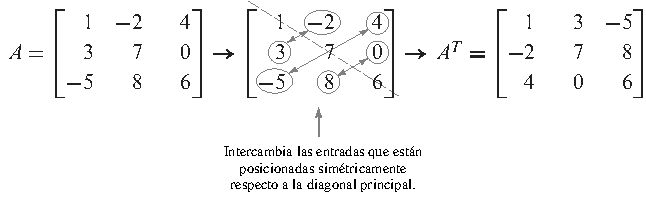
\includegraphics{Images/Capitulo2/Transpuesta.pdf}
\end{matrizn}

\begin{definicion}{}{matriz-antisimetrica}
    Sea $A$ una matriz cuadrada.
    \begin{enumerate}[label=\roman*), topsep=6pt, itemsep=0pt]
        \item Si $A^T = A$, decimos que la matriz $A$ es \emph{simétrica}.
        \item Si $A^T = -A$, decimos que la matriz $A$ es \emph{antisimétrica}.
    \end{enumerate}
\end{definicion}

\begin{examplebox}{}{}
    Consideremos
    $$A = \begin{bmatrix}
        1 & 3 \\
        3 & 1
    \end{bmatrix}.$$
    Notemos que $A^T = A$, por lo que $A$ es simétrica. Sin embargo, si consideramos
    $$B = \begin{bmatrix*}[r]
        0 & 2 \\
        -2 & 0
    \end{bmatrix*}.$$
    Notemos que $B^T = - B$, por lo que $B$ es antisimétrica.
\end{examplebox}

A continuación, se presentan algunas propiedades de la transpuesta que facilitan su manipulación y que se utilizarán en diversos contextos posteriores.

\newpage

\begin{theorem}{}{propiedades_transpuesta}
    Sean $A$ y $B$ matrices, cuyos tamaños son tales que pueden realizarse las operaciones indicadas, y sea $\alpha$ un escalar. Entonces
    \begin{enumerate}[label=\roman*), topsep=6pt, itemsep=0pt]
        \item $\left(A^T\right)^T = A$.
        \item $(A + B)^T = A^T + B^T$.
        \item $(\alpha A)^T = \alpha A^T$.
        \item $(AB)^T = B^TA^T$.
    \end{enumerate}

    \tcblower
    \demostracion Se dejan como ejercicio al lector.
\end{theorem}

La segunda y cuarta propiedad del teorema \ref{theorem:propiedades_transpuesta} pueden generalizarse a sumas y productos de un número finito de matrices. Es decir,
$$(A_1 + A_2 + \cdots + A_k)^T = A_1^T + A_2^T + \cdots + A_k^T \quad \text{ y } \quad (A_1 A_2 \cdots A_k)^T = A_k^T \cdots A_2^T A_1^T$$
si se supone que los tamaños de las matrices son tales que todas las operaciones pueden realizarse.

\begin{theorem}{}{}
    \begin{enumerate}[label=\alph*), topsep=6pt, itemsep=0pt]
        \item Si $A$ es una matriz cuadrada, entonces $A + A^T$ es una matriz simétrica.
        \item Para cualquier matriz $A$, $AA^T$ y $A^TA$ son matrices simétricas.
    \end{enumerate}
\end{theorem}

\begin{definicion}{}{}
    Sea $A \in \mathcalm{M}_{n \times n}(\RR)$, decimos que $A$ es una matriz diagonal si todas sus entradas fuera de la diagonal principal son cero, es decir, $[ a_{ij} ] = 0$, para toda $i \neq j$. Si $[ a_{ij} ] = a_{ij}$, entonces escribiremos $$A = \operatorname{diag} \left\lbrace a_{11}, a_{22}, \dots, a_{nn} \right\rbrace$$
\end{definicion}

\begin{examplebox}{}{}
    Sea
    $$\makecell{\includegraphics[page=26]{Externalizacion/C2/MatricesC2.pdf}}$$
    entonces
    $$A = \operatorname{diag} \{ -1, -6, -9 \}.$$
\end{examplebox}

Las matrices diagonales, constituyen un caso particularmente simple de las matrices cuadradas. Gracias a su estructura, son fáciles de manipular algebraicamente y presentan un comportamiento estable bajo operaciones comunes. Las siguientes propiedades muestran que el conjunto de matrices diagonales es cerrado bajo suma, multiplicación escalar, multiplicación entre matrices y transposición:

\begin{theorem}{}{propiedades_diagonal}
    Sean $A$, $B$ matrices diagonales y sea $\alpha \in \RR$, entonces
    \begin{enumerate}[label=\roman*), topsep=6pt, itemsep=0pt]
        \item $A + B$ es diagonal.
        \item $AB$ es diagonal.
        \item $\alpha A$ es diagonal.
        \item $A^{T} = A$.
    \end{enumerate}

    \tcblower
    \demostracion Se dejan como ejercicio al lector.
\end{theorem}

\begin{definicion}{}{}
    Sea $A$ una matriz cuadrada.
    \begin{enumerate}[label=\roman*), topsep=6pt, itemsep=0pt]
        \item Decimos que $A$ es una matriz triangular superior si todas las entradas bajo la diagonal son cero, es decir, $[ a_{ij} ] = 0$, para toda $i > j$.
        \item decimos que $A$ es una matriz triangular inferior si todas las entradas sobre la diagonal son cero, es decir, $[ a_{ij} ] = 0$, para toda $i < j$.
    \end{enumerate}
\end{definicion}

\newpage

\begin{examplebox}{}{}
    Un ejemplo de una matriz triangular superior es:
    \begin{matrizn}
        \makecell{\includegraphics[page=27]{Externalizacion/C2/MatricesC2.pdf}}
    \end{matrizn}
    Un ejemplo de una matriz triangular inferior es:
    \begin{matrizn}
        \makecell{\includegraphics[page=28]{Externalizacion/C2/MatricesC2.pdf}}
    \end{matrizn}
\end{examplebox}

Las matrices triangulares, ya sean superiores o inferiores, poseen estructuras algebraicamente convenientes que se conservan bajo ciertas operaciones. En el caso de las matrices triangulares superiores, se cumple lo siguiente:

\begin{theorem}{}{}
    Sean $A$, $B$ matrices triangulares superiores y sea $\alpha \in \RR$, entonces
    \begin{enumerate}[label=\roman*), topsep=6pt, itemsep=0pt]
        \item $A + B$ es triangular superior.
        \item $AB$ es triangular superior.
        \item $\alpha A$ es triangular superior.
    \end{enumerate}

    \tcblower
    \demostracion Se dejan como ejercicio al lector.
\end{theorem}

De manera análoga, las matrices triangulares inferiores también son cerradas bajo suma, multiplicación y multiplicación escalar, como se muestra a continuación:

\begin{theorem}{}{}
    Sean $A$, $B$ matrices triangulares inferiores y sea $\alpha \in \RR$, entonces
    \begin{enumerate}[label=\roman*), topsep=6pt, itemsep=0pt]
        \item $A + B$ es triangular inferior.
        \item $AB$ es triangular inferior.
        \item $\alpha A$ es triangular inferior.
    \end{enumerate}

    \tcblower
    \demostracion Se dejan como ejercicio al lector.
\end{theorem}

\section{Sistemas de ecuaciones}

En el estudio de diversos fenómenos, desde problemas físicos y económicos hasta modelos computacionales y redes eléctricas, es común encontrar relaciones entre cantidades desconocidas que se expresan mediante ecuaciones. En muchos casos, estas relaciones tienen una estructura algebraicamente simple: las incógnitas aparecen sin exponentes ni productos entre ellas. A este tipo de expresiones se les conoce como ecuaciones lineales.

\begin{definicion}{}{}
    Sean $a_1, a_2, \dots, a_n, b$ escalares. Una ecuación lineal con $n$ incógnitas es una expresión de la forma
    $$a_1x_1 + a_2x_2 + \cdots + a_nx_n = b,$$
    donde $a_1, a_2, \dots, a_n, b$ se llaman \emph{coeficientes de la ecuación} y $x_1, x_2, \dots, x_n$ se llaman \emph{incógnitas}.
\end{definicion}

Una \emph{solución} de la ecuación lineal anterior es un conjunto de valores de las incógnitas, digamos $x_1 = k_1$, $x_2 = k_2$, $\dots$, $x_n = k_n$, con la propiedad de que es cierta la siguiente expresión (obtenida sustituyendo cada $x_i$ por $k_i$ en la ecuación):
$$a_1 k_1 + a_2 k_2 + \cdots + a_n k_n = b.$$
\newpage\noindent
Se dice entonces que este conjunto de valores \emph{satisface} la ecuación. El conjunto de todas las soluciones se llama \emph{conjunto solución}, \emph{solución general} o, simplemente, la \emph{solución} de la ecuación.

Las nociones anteriores suponen que las incógnitas están ordenadas. Cuando se eviten los subíndices, normalmente utilizaremos variables $x$, $y$, $z$ para denotar tres incógnitas, $x$, $y$, $z$, $t$ para denotar cuatro incógnitas y así sucesivamente.

\begin{examplebox}{}{}
    \begin{enumerate}[label=\alph*), topsep=6pt, itemsep=0pt]
        \item La ecuación $2x - 5y + 3xz = 4$ no es lineal, porque el producto de dos incógnitas es de segundo grado.
        \item La ecuación $x + 2y - 4z + t = 3$ es lineal en las cuatro incógnitas $x, y, z, t$. Una solución a esta ecuación es: $x = 3$, $y = 2$, $z = 1$, $t = 0$. Esto ya que
        $$3 + 2(2) - 4(1) + 0 = 3 \Longrightarrow 3 = 3$$
        es una expresión cierta. Sin embargo: $x = 1$, $y = 2$, $z = 4$, $t = 5$ no es una solución de la ecuación porque
        $$1 + 2(2) - 4(4) + 5 = 3 \Longrightarrow -6 = 3$$
        no es cierto.
    \end{enumerate}
\end{examplebox}

Antes de estudiar sistemas más generales, es útil analizar el caso más simple: una ecuación lineal con una sola incógnita.

\begin{theorem}{}{}
    Consideremos la ecuación lineal $ax = b$.
    \begin{enumerate}[label=\roman*), topsep=6pt, itemsep=0pt]
        \item Si $a \neq 0$, $x = a^{-1}b$ es la solución única de $ax = b$.
        \item Si $a = 0$, pero $b \neq 0$, $ax = b$ no tiene solución.
        \item Si $a = 0$ y $b = 0$, todo escalar $k$ es solución de $ax = b$.
    \end{enumerate}

    \tcblower
    \demostracion
    \begin{enumerate}[label=\roman*), topsep=6pt, itemsep=0pt]
        \item Supongamos $a \neq 0$. Entonces existe el escalar $a^{-1}b$. Sustituyendo $a^{-1}b$ en $ax = b$ se obtiene $a(a^{-1}b) = b$, o bien $b = b$; por consiguiente, $a^{-1}b$ es una solución. Por otra parte, supongamos que $x_0$ es solución de $ax = b$, de forma que $ax_0 = b$. Multiplicando ambos miembros por $a^{-1}$ se obtiene $x_0 = a^{-1}b$. De aquí $a^{-1}b$ es la única solución de $ax = b$.
        \newpage
        \item Sea ahora, $a = 0$. Entonces, para todo escalar $k$, tenemos $ak = 0k = 0$. Si $b \neq 0$, $ax \neq b$. De acuerdo con esto, $k$ no es solución de $ax = b$.
        \item Si $b = 0$, $ak = b$. Esto es, cualquier escalar $k$ es una solución de $ax = b$.
    \end{enumerate}
\end{theorem}

Una ecuación lineal se dice \textit{degenerada} si tiene la forma
$$0x_1 + 0x_2 + \cdots + 0x_n = b$$
esto es, si cada coeficiente es igual a cero. En este caso, el comportamiento de la ecuación depende únicamente del valor del término independiente $b$. Si $b \neq 0$, la ecuación se reduce a una contradicción del tipo $0 = b$, por lo que no tiene solución. En cambio, si $b = 0$, la igualdad se cumple para cualquier vector $\mathbb{x} \in \RR[n]$, y por tanto, todo vector es solución.

\begin{definicion}{}{}
    Consideremos la ecuación lineal no degenerada
    $$a_1x_1 + a_2x_2 + \cdots + a_nx_n = b.$$
    Por \emph{primera incógnita} en dicha ecuación, entendemos la primera con coeficiente no nulo. Su posición $p$ en la ecuación es entonces el menor entero de $j$ para el cual $a_j \neq 0$. Es decir, $x_p$ es la primer incógnita si $a_j = 0$ para $j < p$, pero $a_p \neq 0$.
\end{definicion}

\begin{examplebox}{}{}
    Consideremos la ecuación lineal $5y - 2z = 3$. Aquí $y$ es la primera incógnita. Si las incógnitas son $x$, $y$ y $z$, entonces $p = 2$ es su posición, pero si $y$ y $z$ son las únicas incógnitas, es $p = 1$.
\end{examplebox}

\begin{theorem}{}{}
    Consideremos una ecuación lineal no degenerada
    $$a_1x_1 + a_2x_2 + \cdots + a_nx_n = b$$
    con primer incógnita $x_p$.
    \begin{enumerate}[label=\roman*), topsep=6pt, itemsep=0pt]
        \item Cualquier conjunto de valores de las incógnitas $x_j$ con $j \neq p$ dará una única solución de la ecuación. Las incógnitas $x_j$ de llaman \emph{variables libres} porque se les puede asignar cualquier valor.
        \item Toda solución de la ecuación se obtiene en el inciso anterior. El conjunto de todas las soluciones se llama \emph{solución general} de la ecuación.
    \end{enumerate}
\end{theorem}

\begin{examplebox}{}{}
    Encuentre dos soluciones particulares y la solución general de la ecuación lineal:
    $$2x - 4y + z = 8.$$

    \tcblower
    \solucion Aquí $x$ es la primera incógnita. De acuerdo con ello, asignamos valores cualesquiera a las variables libres $y$ y $z$, entonces despejamos $x$ para obtener una solución. Por ejemplo, si tomamos $y = 1$ y $z = 0$, la sustitución en la ecuación proporciona
    $$2x - 4(1) + 0 = 8 \Longrightarrow x = 6.$$
    Por lo tanto, una solución es:
    $$x = 6, \quad y = 1, \quad z = 0.$$
    Ahora bien, si tomamos $y = 3$ y $z = 4$, la sustitución en la ecuación proporciona
    $$2x - 4(3) + 4 = 8 \Longrightarrow x = 8.$$
    Por lo tanto, otra solución es:
    $$x = 8, \quad y = 3, \quad z = 4.$$
    La solución general de la ecuación principal, se obtiene como sigue: En primer lugar, asignamos valores arbitrarios (llamados \textit{parámetros}) a las variables libres, digamos $y = a$ y $z = b$. A continuación sustituimos en la ecuación para obtener
    $$2x - 4a + b = 8,$$
    o equivalentemente
    $$x = 4 + 2a - \frac{1}{2}b.$$
    Entonces
    $$x = 4 + 2a - \frac{1}{2}b, \quad y = a, \quad z = b$$
    es la solución general.
\end{examplebox}

\begin{definicion}{}{JSJJNDJUDUDJNDN}
    Sea $A \in \mathcalm{M}_{n \times n}(\RR)$ y $\mathbb{x} \in \RR[n]$, se define el producto de la matriz $A$ con el vector $\mathbb{x}$ como:
    $$\makecell{\includegraphics[page=29]{Externalizacion/C2/MatricesC2.pdf}}$$
\end{definicion}

\newpage

\begin{definicion}{}{}
    Si $A\mathbb{x} = \mathbb{b}$, obtenemos
    \begin{equation}
        \begin{aligned}
            a_{11}x_1 + a_{12}x_2 + \cdots + a_{1n}x_n & = b_1 \\
            a_{21}x_1 + a_{22}x_2 + \cdots + a_{2n}x_n & = b_2 \\
            \vdots \hspace{1cm}  \\
            a_{m1}x_1 + a_{m2}x_2 + \cdots + a_{mn}x_n & = b_m
        \end{aligned} \label{ec29}
    \end{equation}
    A la expresión \eqref{ec29} se le llamará \emph{sistema de ecuaciones lineales} (SEL) de $m$ ecuaciones con $n$ incógnitas. Además, si $\mathbb{b} = \mathbb{0}$, obtenemos
    \begin{equation*}
        \begin{aligned}
            a_{11}x_1 + a_{12}x_2 + \cdots + a_{1n}x_n & = 0 \\
            a_{21}x_1 + a_{22}x_2 + \cdots + a_{2n}x_n & = 0 \\
            \vdots \hspace{1cm}  \\
            a_{m1}x_1 + a_{m2}x_2 + \cdots + a_{mn}x_n & = 0
        \end{aligned}
    \end{equation*}
    A esta expresión se le llamará \emph{sistema homogéneo}.
\end{definicion}

Observemos que en la definición \ref{definicion:JSJJNDJUDUDJNDN} se puso a $\mathbb{x}$ como una matriz de tamaño $n \times 1$, cuando al principio de dicha definición se dijo que pertenecía a $\RR[n]$. Aunque pueda parecer un error, no es así, pues $\mathbb{x}$ se puede representar de ambas maneras, sea como vector o como matriz de tamaño $n \times 1$. Así que si $\mathbb{x} \in \RR[n]$, entonces $\mathbb{x} \in \mathcalm{M}_{n \times 1}(\RR)$. Cuando consideremos a $\mathbb{x} \in \mathcalm{M}_{n \times 1}(\RR)$, escribiremos a $\mathbb{x}$ como
$$\makecell{\includegraphics[page=30]{Externalizacion/C2/MatricesC2.pdf}}$$
Esto nos será de gran ayuda para entender de mejor manera los sistemas de ecuaciones lineales y no confundirnos con la notación.

\marginElement{
\begin{flushleft}
    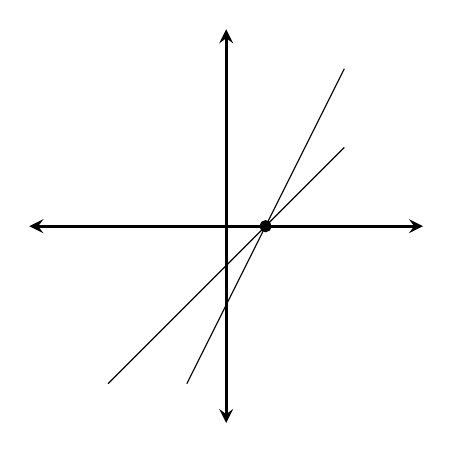
\begin{tikzpicture}
        \draw[black,stealth-stealth,very thick] (0,0) -- (5,0);
        \draw[black,stealth-stealth,very thick] (2.5,-2.5) -- (2.5,2.5);
        \draw (1,-2) -- (4,1);
        \draw (2,-2) -- (4,2);
        \filldraw (3,0) circle (2pt);
        %\node at (0,7) {~};
    \end{tikzpicture}
    {\normalsize\TituloBox{i)} Sistemas con única solución}
\end{flushleft}
~\vspace{-1cm}
\begin{flushleft}
    \begin{tikzpicture}
        \draw[black,stealth-stealth,very thick] (0,0) -- (5,0);
        \draw[black,stealth-stealth,very thick] (2.5,-2.5) -- (2.5,2.5);
        \draw[thick] (1,-2) -- (4,2);
        \draw (1,-2) -- (4,2);
    \end{tikzpicture}
    {\normalsize\TituloBox{ii)} Sistemas con infinitas soluciones}
\end{flushleft}
~\vspace{-1cm}
\begin{flushleft}
    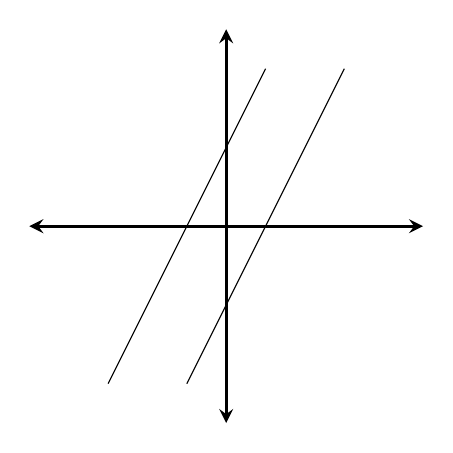
\begin{tikzpicture}
        \draw[black,stealth-stealth,very thick] (12,0) -- (17,0);
        \draw[black,stealth-stealth,very thick] (14.5,-2.5) -- (14.5,2.5);
        \draw (13,-2) -- (15,2);
        \draw (14,-2) -- (16,2);
    \end{tikzpicture}
    {\normalsize\TituloBox{iii)} Sistemas sin solución}
\end{flushleft}
~\vspace{-0.5cm}
\captionsetup*[figure]{font={normalsize},hypcap=false}%
\captionof{figure}{Representación de los posibles casos del conjunto solución de un SEL $2 \times 2$}\label{JWISIKSJSKISOOKKOOOOIUKKSK}
}

Consideremos inicialmente un sistema de dos ecuaciones lineales con dos incógnitas $x_1$ y $x_2$:
\begin{align*}
    a_{11}x_1 + a_{12}x_2 & = b_1 \\ 
    a_{21}x_1 + a_{22}x_2 & = b_2
\end{align*}
donde $a_{11}$, $a_{12}$, $a_{21}$, $a_{22}$, $b_1$, y $b_2$ son coeficientes reales. Geométricamente, cada ecuación representa una recta en el plano cartesiano, y la solución del sistema corresponde a sus puntos de intersección. Este sistema admite tres escenarios posibles: solución única (rectas que se cortan en un punto), infinitas soluciones (rectas coincidentes), o ninguna solución (rectas paralelas no coincidentes), como ilustra la figura \ref{JWISIKSJSKISOOKKOOOOIUKKSK}.

Al extender este concepto al espacio tridimensional, obtenemos un sistema de tres ecuaciones con tres incógnitas $x_1$, $x_2$, y $x_3$:
\begin{align*}
    a_{11}x_1 + a_{12}x_2 + a_{13}x_3 & = b_1 \\ 
    a_{21}x_1 + a_{22}x_2 + a_{23}x_3 & = b_2 \\ 
    a_{31}x_1 + a_{32}x_2 + a_{33}x_3 & = b_3
\end{align*}
donde los coeficientes $a_{ij}$ y términos independientes $b_k$ son números reales. En este caso, cada ecuación describe un plano en el espacio tridimensional, y la solución representa la intersección de estos planos. Análogamente al caso bidimensional, el sistema puede tener: solución única (tres planos que se intersectan en un punto), infinitas soluciones (planos coincidentes o que se cortan formando una recta), o ninguna solución (planos paralelos o sin intersección común). Aunque la visualización geométrica tridimensional es más compleja, la figura \ref{KSKJSJSJJJJSJSJJSDDDD} muestra una representación simplificada de estos posibles casos.
\newpage
\begin{figure*}[h!]
    \centering
    \subfloat[Tres planos se intersecan en un solo punto]{
    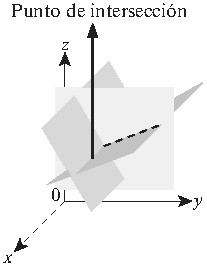
\includegraphics[height=0.4\textwidth]{Images/Capitulo2/Plano111.pdf}
    }\hfill
    \subfloat[Tres planos se intersecan en la misma recta]{
    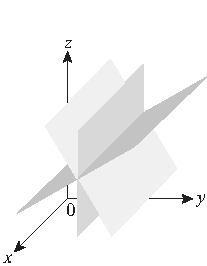
\includegraphics[height=0.4\textwidth]{Images/Capitulo2/Plano222.pdf}
    }\hfill
    \subfloat[Dos planos se intersecan en una recta]{
    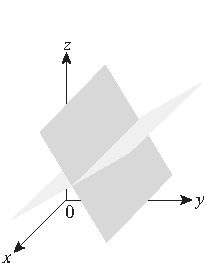
\includegraphics[height=0.4\textwidth]{Images/Capitulo2/Plano333.pdf}
    } \hfill
    \subfloat[Los planos paralelos no tienen puntos en común]{
    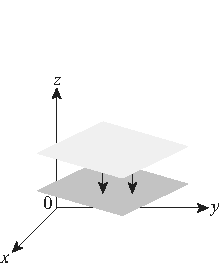
\includegraphics[height=0.4\textwidth]{Images/Capitulo2/Plano444.pdf}
    }
    \caption{Representación de los posibles casos del conjunto solución de un SEL $3 \times 3$}\label{KSKJSJSJJJJSJSJJSDDDD}
\end{figure*}

La figura \ref{KSKJSJSJJJJSJSJJSDDDD} ilustra cómo interactúan los planos en un sistema de tres ecuaciones lineales con tres incógnitas. Cada caso refleja una relación distinta entre las ecuaciones, lo que determina si el sistema tiene una solución única, infinitas soluciones o ninguna.

Por último, este análisis geométrico sirve como base para introducir nociones más abstractas, como el núcleo y la imagen de una matriz, que exploraremos en la siguiente sección. Estas ideas no solo son esenciales para resolver sistemas, sino también para comprender mejor las estructuras que los sustentan.

\section{Núcleo e imagen de una matriz}

\begin{definicion}{}{}
    Sea $A \in \matrizmn$, se define el \emph{espacio nulo} de $A$, denotado por $\mathcalm{N}(A)$, como:
    $$\mathcalm{N}(A) = \left\{ \mathbb{x} \in \RR[n] \mid A\mathbb{x} = \mathbb{0} \in \RR[m] \right\}$$
    Al espacio nulo de $A$ también de le llama \emph{kernel} de $A$, o bien, \emph{núcleo} de $A$.
\end{definicion}

\begin{theorem}{}{}
    Sea $A \in \matrizmn$, entonces $\mathcalm{N}(A)$ es un subespacio de $\RR[n]$.

    \tcblower
    \demostracion
    \begin{enumerate}[label=\roman*), topsep=6pt, itemsep=0pt]
        \item Sean $\mathbb{x}$, $\mathbb{y} \in \mathcalm{N}(A)$, entonces
        \begin{equation*}
            A\mathbb{x} = \mathbb{0} \quad \text{ y } \quad A\mathbb{y} = \mathbb{0} \label{ec30}
        \end{equation*}
        Ahora
        \begin{align*}
            A(\mathbb{x} + \mathbb{y}) & = A \mathbb{x} + A \mathbb{y} \\
            & = \mathbb{0} + \mathbb{0} \\
            & = \mathbb{0}
        \end{align*}
        Entonces $\mathbb{x} + \mathbb{y} \in \mathcalm{N}(A)$. Por tanto, se cumple la propiedad de cerradura para la suma.
        \item Se deja como ejercicio al lector.
    \end{enumerate}
    De (i) y (ii), se sigue que $\mathcalm{N}(A)$ es subespacio de $\RR[n]$.
\end{theorem}

\begin{definicion}{}{}
    Llamaremos \emph{nulidad} de $A$, denotada por $\nu(A)$, a la dimensión del espacio nulo, es decir,
    $$\nu(A) = \Dim\big(\mathcalm{N}(A)\big).$$
\end{definicion}

\newpage

\begin{examplebox}{}{}
    Determine $\mathcalm{N}(A)$ y $\nu(A)$ de la siguiente matriz
    $$A = \begin{bmatrix*}[r]
        1 & 2 & -1 \\
        2 & -1 & 3
    \end{bmatrix*}$$

    \tcblower
    \solucion Por definición,
    \begin{matrizn}
        \makecell{\includegraphics[page=31]{Externalizacion/C2/MatricesC2.pdf}}
    \end{matrizn}
    Entonces
    \begin{align*}
        x_1 + 2x_2 - x_3 & = 0\\
        2x_1 - x_2 + 3x_3 & = 0
    \end{align*}
    Multiplicando la segunda ecuación por $2$, obtenemos
    \begin{align*}
        x_1 + 2x_2 - x_3 & = 0\\
        4x_1 - 2x_2 + 6x_3 & = 0
    \end{align*}
    Sumando la primer ecuación con la segunda, obtenemos
    $$5x_1 + 5x_3 = 0$$
    Por tanto, $x_3 = -x_1$. Sustituyendo en la primer ecuación, obtenemos
    $$2x_1 + 2x_2 = 0$$
    Por tanto, $x_2 = -x_1$. Se sigue entonces
    \begin{matrizn}
        \makecell{\includegraphics[page=32]{Externalizacion/C2/MatricesC2.pdf}}
    \end{matrizn}
    Por tanto, $\mathcalm{N}(A) = \Gen \left( \left\{ \begin{pNiceMatrix}[cell-space-limits=3pt,r]
        \vphantom{^A}1 \\
        -1 \\
        -1\vphantom{_A}
    \end{pNiceMatrix} \right\} \right)$. Además, $\nu(A) = 1$.
\end{examplebox}

Si $A$ es la matriz cero de tamaño $m \times n$, entonces el sistema se convierte en
$$\mathbb{0}_{m \times n} \mathbb{x} = \mathbb{0}_{n \times 1}.$$
Dado que la matriz cero anula cualquier vector $\mathbb{x} \in \RR[n]$, el sistema siempre tiene todas las soluciones posibles en $\RR[n]$. Esto significa que el espacio nulo de $\mathbb{0}_{m \times n}$ es todo el espacio $\RR[n]$
$$\mathcalm{N}(\mathbb{0}) = \RR[n] \quad \text{ y } \quad \nu(\mathbb{0}) = n.$$
\newpage
%Dado que $\mathcalm{N}(\mathbb{0}) = \RR[n]$, su dimensión es $n$. Es decir,
%$$\nu(\mathbb{0}) = n.$$

\begin{examplebox}{}{}
    Determine $\mathcalm{N}(A)$ y $\nu(A)$ de la siguiente matriz
    $$A = \begin{bmatrix*}[r]
        1 & 2 \\
        1 & -1
    \end{bmatrix*}$$

    \tcblower
    \solucion Por definición,
    \begin{align*}
        \mathcalm{N}(A) & = \left\{ \mathbb{x} \in \RR[2] \mid A\mathbb{x} = \mathbb{0} \in \RR[2] \right\} \\
        & = \left\{ \begin{pmatrix}
            x_1 \\
            x_2
        \end{pmatrix} \in \RR[2] \mid \begin{bmatrix*}[r]
            1 & 2 \\
            1 & -1
        \end{bmatrix*} \begin{bmatrix}
            x_1 \\
            x_2
        \end{bmatrix} = \begin{bmatrix}
            0 \\
            0
        \end{bmatrix} \right\} \\
        & = \left\{ \begin{pmatrix}
            x_1 \\
            x_2
        \end{pmatrix} \in \RR[2] \mid \begin{bmatrix}
            x_1 + 2x_2 \\
            x_1 - x_2
        \end{bmatrix} = \begin{bmatrix}
            0 \\
            0
        \end{bmatrix} \right\}
    \end{align*}
    Entonces
    \begin{align*}
        x_1 + 2x_2 = 0\\
        x_1 - x_2 = 0
    \end{align*}
    Restando la primer ecuación de la segunda, obtenemos que
    $$3x_2 = 0 \Longrightarrow x_2 = 0$$
    y sustituyendo en la segunda ecuación se obtiene que
    $$x_1 = 0$$
    Se sigue entonces que
    $$x_1 = 0 \quad \text{ y } \quad x_2 = 0$$
    por lo que
    \begin{align*}
        \mathcalm{N}(A) & = \left( \left\{ \begin{pmatrix}
            0 \\
            0
        \end{pmatrix} \right\} \right) \\
        & = \Gen \left( \left\{ \begin{pmatrix}
            0 \\
            0
        \end{pmatrix} \right\} \right)
    \end{align*}
    Por tanto, $\mathcalm{N}(A) = \Gen \left( \left\{ \begin{pmatrix}
        0 \\
        0
    \end{pmatrix} \right\} \right)$. Además, $\nu(A) = 0$.
\end{examplebox}

\begin{definicion}{}{}
    Sea $A \in \matrizmn$, se define la \emph{imagen} de $A$, denotado por $\mathcalm{R}(A)$, como
    $$\mathcalm{R}(A) = \left\{ \mathbb{y} \in \RR[m] \mid A\mathbb{x} = \mathbb{y}, \text{ para algún } \mathbb{x} \in \RR[n] \right\}$$
\end{definicion}

\begin{theorem}{}{}
    Sea $A \in \matrizmn$, entonces $\mathcalm{R}(A)$ es un subespacio de $\RR[m]$

    \tcblower
    \demostracion
    \begin{enumerate}[label=\roman*), topsep=6pt, itemsep=0pt]
        \item Sean $\mathbb{y}_1$, $\mathbb{y}_2 \in \mathcalm{R}(A)$, entonces
        \begin{equation}
            A\mathbb{x}_1 = \mathbb{y}_1, \text{ para algún } \mathbb{x}_1 \in \RR[n] \label{UYHDFHDFVFDVFVHFD}
        \end{equation}
        y
        \begin{equation}
            A\mathbb{x}_2 = \mathbb{y}_2, \text{ para algún } \mathbb{x}_2 \in \RR[n] \label{HFHDVJHFHJUGHHFGJ}
        \end{equation}
        Así, de las expresiones \eqref{UYHDFHDFVFDVFVHFD} y \eqref{HFHDVJHFHJUGHHFGJ},
        \begin{align*}
            \mathbb{y}_1 + \mathbb{y}_2 & = A\mathbb{x}_1 + A\mathbb{x}_2 \\
            & = A(\mathbb{x}_1 + \mathbb{x}_2) \\
            & = A\mathbb{w}
        \end{align*}
        siendo $\mathbb{w} = \mathbb{x}_1 + \mathbb{x}_2$. Por tanto, $\mathbb{y}_1 + \mathbb{y}_2 \in \mathcalm{R}(A)$, es decir, se cumple la cerradura bajo la suma.
        \item Se deja como ejercicio al lector.
    \end{enumerate}
    De (i) y (ii), se sigue que $\mathcalm{R}(A)$ es un subespacio de $\RR[m]$.
\end{theorem}

\begin{definicion}{}{}
    Llamaremos \emph{rango} de $A$, denotado por $\rho(A)$, a la dimensión de la imagen, es decir,
    $$\rho(A) = \Dim\big(\mathcalm{R}(A)\big)$$
\end{definicion}

\begin{examplebox}{}{}
    Determine $\mathcalm{R}(A)$ y $\rho(A)$ de la siguiente matriz
    $$A = \begin{bmatrix*}[r]
        1 & 2 \\
        1 & -1
    \end{bmatrix*}$$

    \tcblower
    \solucion Por definición,
    \begin{align*}
        \mathcalm{R}(A) & = \left\{ \mathbb{y} \in \RR[2] \mid A\mathbb{x} = \mathbb{y}, \text{ para algún } \mathbb{x} \in \RR[2] \right\} \\
        & = \left\{ \begin{pmatrix}
            y_1 \\
            y_2
        \end{pmatrix} \in \RR[2] \mid \begin{bmatrix*}[r]
            1 & 2 \\
            1 & -1
        \end{bmatrix*} \begin{bmatrix}
            x_1 \\
            x_2
        \end{bmatrix} = \begin{bmatrix}
            y_1 \\
            y_2
        \end{bmatrix}, \text{ para algún } \mathbb{x} \in \RR[2] \right\} \\
        & = \left\{ \begin{pmatrix}
            y_1 \\
            y_2
        \end{pmatrix} \in \RR[2] \mid \begin{bmatrix}
            x_1 + 2x_2 \\
            x_1 - x_2
        \end{bmatrix} = \begin{bmatrix}
            y_1 \\
            y_2
        \end{bmatrix}, \text{ para algún } \mathbb{x} \in \RR[2] \right\} \\
        & = \left\{ \begin{pmatrix}
            y_1 \\
            y_2
        \end{pmatrix} = x_1 \begin{pmatrix}
            1 \\
            1
        \end{pmatrix} + x_2 \begin{pmatrix*}[r]
            2 \\
            -1
        \end{pmatrix*} \mid x_1, x_2 \in \RR \right\} \\
        & = \Gen \left(\left\{ \begin{pmatrix}
            1 \\
            1
        \end{pmatrix}, \begin{pmatrix*}[r]
            2 \\
            -1
        \end{pmatrix*} \right\}\right)
    \end{align*}
    Observemos que el conjunto de vectores anterior es linealmente independiente. Por tanto, $\mathcalm{R}(A) = \Gen \left(\left\{ \begin{pmatrix}
        1 \\
        1
    \end{pmatrix}, \begin{pmatrix*}[r]
        2 \\
        -1
    \end{pmatrix*} \right\}\right)$ y $\rho(A) = 2$.
\end{examplebox}

\begin{examplebox}{}{matrizrangoe}
    Determine $\mathcalm{R}(A)$ y $\rho(A)$ de la siguiente matriz
    $$A = \begin{bmatrix*}[r]
        1 & 2 & -1 \\
        2 & -1 & 3
    \end{bmatrix*}$$

    \tcblower
    \solucion Por definición,
    \begin{matrizn}
        \makecell{\includegraphics[page=33]{Externalizacion/C2/MatricesC2.pdf}}
    \end{matrizn}
    Observemos que el conjunto anterior de vectores no es linealmente independiente, pues el primer vector puede expresarse como combinación lineal de los otros dos. En particular, si denotamos los vectores respectivamente como $\mathbb{v}_1$, $\mathbb{v}_2$, $\mathbb{v}_3$, entonces existen escalares $\alpha = 1$ y $\beta = 1$ tales que $\mathbb{v}_1 = \alpha \mathbb{v}_2 + \beta \mathbb{v}_3$. Por tanto, esto implica que $\mathcalm{R}(A) = \Gen \left(\left\{ \begin{pmatrix*}[r]
        2 \\
        -1
    \end{pmatrix*}, \begin{pmatrix*}[r]
        -1 \\
        3
    \end{pmatrix*} \right\}\right)$ y $\rho(A) = 2$.
\end{examplebox}

\newpage

\begin{definicion}{}{}
    Si $A \in \matrizmn$, sean $\{ \mathbb{r}_1, \mathbb{r}_2, \dots, \mathbb{r}_m \}$ los renglones de $A$ y $\{ \mathbb{c}_1, \mathbb{c}_2, \dots, \mathbb{c}_n \}$ las columnas de $A$. Es decir,
    \begin{matrizn}
        \makecell{\includegraphics[page=34]{Externalizacion/C2/MatricesC2.pdf}}
    \end{matrizn}
    Definimos el espacio renglón de $A$, denotado por $R_A$, como
    $$R_A = \Gen (\{ \mathbb{r}_1, \mathbb{r}_2, \dots, \mathbb{r}_m \}) \subseteq \RR[n]$$
    y el espacio columna, denotado por $C_A$, como
    $$C_A = \Gen (\{ \mathbb{c}_1, \mathbb{c}_2, \dots, \mathbb{c}_n \}) \subseteq \RR[m]$$
\end{definicion}

\begin{theorem}{}{}
    La imagen de una matriz es igual al espacio columna.

    \tcblower
    \demostracion Para demostrar que $C_A = \mathcalm{R}(A)$, tenemos que demostrar que $\mathcalm{R}(A) \subseteq C_A$ e $C_A \subseteq \mathcalm{R}(A)$.
    \begin{enumerate}[label=\roman*), topsep=6pt, itemsep=0pt]
        \item Queremos probar que $\mathcalm{R}(A) \subseteq C_A$. Supongamos que $\mathbb{y} \in \mathcalm{R}(A)$. Entonces existe un vector $\mathbb{x}$ tal que $\mathbb{y} = A\mathbb{x}$, pero podemos expresa a $A\mathbb{x}$ como una combinación lineal de las columnas de $A$. Para ver esto, consideremos
        \begin{matrizn}
            \makecell{\includegraphics[page=35]{Externalizacion/C2/MatricesC2.pdf}}
        \end{matrizn}
        Entonces
        \begin{matrizn}
            \makecell{\includegraphics[page=36]{Externalizacion/C2/MatricesC2.pdf}}
        \end{matrizn}
        y por consiguiente,
        \begin{matrizn}
            \makecell{\includegraphics[page=37]{Externalizacion/C2/MatricesC2.pdf}}
        \end{matrizn}
        Por lo tanto, $\mathbb{y} \in C_A$, de manera que $\mathcalm{R}(A) \subseteq C_A$.
        \item Se deja como ejercicio al lector.
    \end{enumerate}
\end{theorem}

Si $A$ es la matriz cero de tamaño $m \times n$, entonces el sistema se convierte en
$$\mathbb{0}_{m \times n} \mathbb{x} = \mathbb{y}.$$
Es decir, la única salida posible es el vector cero en $\RR[m]$. Esto implica que
$$\mathcalm{R}(\mathbb{0}) = \{\mathbb{0}_m\}.$$
Esto significa que la imagen de la matriz cero es el subespacio trivial $\{\mathbb{0}_m\}$ en $\RR[m]$. Dado que $\mathcalm{R}(\mathbb{0}) = \{\mathbb{0}_m\}$, su dimensión es 0. Es decir,
$$\rho(\mathbb{0}) = 0.$$

\newpage

\begin{theorem}{}{}
    Si $A$ es una matriz de $m \times n$, entonces
    $$\dim R_A = \dim C_A = \dim\big(\mathcalm{R}(A)\big) = \rho(A)$$

    \tcblower
    \demostracion Denotaremos por $\alpha_{ij}$ la componente $ij$ de $A$. Debemos demostrar que $\dim R_A = \dim C_A$. Los renglones de $A$ se denotan por $\mathbb{r}_1, \mathbb{r}_2, \dots, \mathbb{r}_m$ y sea $k = \dim R_A$. Sea $S = \{\mathbb{s}_1, \mathbb{s}_2, \dots, \mathbb{s}_k\}$ una base para $R_A$. Entonces cada renglón de $A$ se puede expresar como una combinación lineal de los vectores en $S$, y se tiene, para algunas constantes $\alpha_{ij}$,
    \begin{equation}
        \begin{aligned}
            \mathbb{r}_1 & = \alpha_{11} \mathbb{s}_1 + \alpha_{12} \mathbb{s}_2 + \cdots + \alpha_{1k} \mathbb{s}_k \\
            \mathbb{r}_2 & = \alpha_{21} \mathbb{s}_1 + \alpha_{22} \mathbb{s}_2 + \cdots + \alpha_{2k} \mathbb{s}_k \\
            \vdots \\
            \mathbb{r}_m & = \alpha_{m1} \mathbb{s}_1 + \alpha_{m2} \mathbb{s}_2 + \cdots + \alpha_{mk} \mathbb{s}_k
        \end{aligned} \label{ec:rengA5}
    \end{equation}
    Ahora la componente $j$ de $\mathbb{r}_i$ es $a_{ij}$. Entonces si se igualan las componentes $j$ de ambos lados de \eqref{ec:rengA5}, se obtiene
    $$\makecell{\includegraphics[page=38]{Externalizacion/C2/MatricesC2.pdf}}$$
    Es decir,
    \begin{matriz}
        \makecell{\includegraphics[page=39]{Externalizacion/C2/MatricesC2.pdf}} \label{ec:rengA6}
    \end{matriz}
    Entonces como el lado izquierdo de \eqref{ec:rengA6} es la columna $j$ de $A$, se observa que cada columna de $A$ se puede escribir como una combinación lineal de $\mathbb{u}_1, \mathbb{u}_2, \dots, \mathbb{u}_k$, lo que significa que los vectores $\mathbb{u}_1, \mathbb{u}_2, \dots, \mathbb{u}_k$ generan a $C_A$ y
    \begin{equation}
        \dim C_A \leq k = \dim R_A. \label{ec:rengA7}
    \end{equation}
    Pero la ecuación \eqref{ec:rengA7} se cumple para cualquier matriz $A$, y en particular para $A^T$. Pero $C_{A^T} = R_A$ y $R_{A^T} = C_A$. Como de \eqref{ec:rengA7} $\dim C_{A^T} \leq \dim R_{A^T}$, se tiene
    \begin{equation}
        \dim R_A \leq \dim C_A. \label{ec:rengA8}
    \end{equation}
    Combinando \eqref{ec:rengA7} y \eqref{ec:rengA8} la demostración queda completa.
\end{theorem}

\begin{examplebox}{}{}
    Tomando la matriz del ejemplo \ref{examplebox:matrizrangoe}, tenemos que
    $$\makecell{\includegraphics[page=40]{Externalizacion/C2/MatricesC2.pdf}}$$
    De acuerdo con el teorema demostrado previamente, tenemos que
    $$\dim R_A = \dim C_A = \dim\big(\mathcalm{R}(A)\big) = \rho(A)$$
    En este caso particular, se verifica que $\dim R_A = \dim C_A = \dim\big(\mathcalm{R}(A)\big) = 2$.
\end{examplebox}

El siguiente teorema establece una relación fundamental entre el rango y la nulidad de una matriz.

\newpage

\begin{theorem}{}{}
    Si $A$ es una matriz con $n$ columnas, entonces
    \begin{equation}
        \rho(A) + \nu(A) = n. \label{ec:rplusn}
    \end{equation}
\end{theorem}

De lo visto anteriormente, hay seis espacios vectoriales importantes asociados con una matriz $A$ y $A^T$:
$$\begin{array}{ll}
    \text{espacio renglón de } A & \qquad\text{espacio renglón de } A^T \\
    \text{espacio columna de } A & \qquad\text{espacio columna de } A^T \\
    \text{espacio nulo de } A & \qquad\text{espacio nulo de } A^T
\end{array}$$
Sin embargo, transponer una matriz convierte los vectores renglón en vectores columna y viceversa,  
por lo tanto, salvo por una diferencia de notación, el espacio renglón de $A^T$ es el mismo que el espacio columna de $A$, y el espacio columna de $A^T$ es el mismo que el espacio renglón de $A$. Así, de los seis espacios mencionados anteriormente, solo los siguientes cuatro son distintos:
$$\begin{array}{ll}
    \text{espacio renglón de } A & \qquad\text{espacio columna de } A \\
    \text{espacio nulo de } A & \qquad\text{espacio nulo de } A^T
\end{array}$$
A estos se les llama los \textit{espacios fundamentales} de una matriz $A$. Ahora consideraremos cómo se relacionan estos cuatro subespacios.

Pongamos atención por un momento en la matriz $A^T$. Como el espacio renglón y el espacio columna de una matriz tienen la misma dimensión, y como al transponer una matriz se intercambian sus columnas por filas y sus filas por columnas, el siguiente resultado no debería ser sorprendente.
\begin{theorem}{}{rangoaat}
    Si $A$ es cualquier matriz, entonces
    $$\rho(A) = \rho\left(A^T\right).$$

    \tcblower
    \demostracion Es evidente, pues $\rho(A) = \dim(R_A) = \dim(C_{A^T}) = \rho\left(A^T\right)$.
\end{theorem}

Este resultado tiene algunas implicaciones importantes. Por ejemplo, si $A$ es una matriz $m \times n$, entonces al aplicar la fórmula \eqref{ec:rplusn} a la matriz $A^T$ y usando el hecho de que esta matriz tiene $m$ columnas, se obtiene
$$\rho\left(A^T\right) + \nu\left(A^T\right) = m$$
lo cual, en virtud del teorema \ref{theorem:rangoaat}, se puede reescribir como
$$\rho(A) + \nu\left(A^T\right) = m.$$
Esta forma alternativa de la fórmula \eqref{ec:rplusn} permite expresar las dimensiones de los cuatro espacios fundamentales en términos del tamaño y el rango de $A$. Específicamente, si $\rho(A) = r$, entonces
\begin{equation}
    \begin{aligned}
        \dim(R_A) & = r & \dim(C_A) & = r \\
        \dim\big(\mathcalm{N}(A)\big) & = n - r & \qquad\dim\left(\mathcalm{N}\left(A^T\right)\right) & = m - r
    \end{aligned} \label{ec:formulasdimensiones}
\end{equation}
Las cuatro fórmulas en \eqref{ec:formulasdimensiones} proporcionan una relación \textit{algebraica} entre el tamaño de una matriz y las dimensiones de sus espacios fundamentales.

\begin{examplebox}{}{}
    ¿Cuál es el rango máximo posible de una matriz $m \times n$ que no es cuadrada?

    \tcblower
    \solucion Dado que los vectores renglón de $A$ pertenecen a $\RR[n]$ y los vectores columna a $\RR[m]$, el espacio renglón de $A$ tiene como máximo dimensión $n$ y el espacio columna como máximo dimensión $m$. Como el rango de $A$ es la dimensión común de su espacio renglón y su espacio columna, se deduce que el rango es como máximo el menor entre $m$ y $n$. Esto se expresa como: $\rho(A) \leq \min(m, n)$.
\end{examplebox}

\newpage

\section{Operaciones elementales en los renglones de una matriz}

Las operaciones elementales por renglón son un conjunto de tres operaciones básicas que se pueden aplicar a los renglones de una matriz sin alterar el espacio renglón de la misma. Estas operaciones son fundamentales en el álgebra lineal para simplificar matrices y resolver sistemas de ecuaciones lineales. La idea principal es manipular la matriz de manera sistemática para alcanzar una forma más sencilla, como la forma escalonada o la forma escalonada reducida, lo que facilita el análisis de sus propiedades. Así, dada una matriz, las operaciones elementales son:
\begin{itemize}
    \item \textbf{Intercambiar dos renglones:} Si intercambiamos los renglones $i$ y $j$, escribiremos $\mathbb{r}_i \rightleftarrows \mathbb{r}_j$.
    \item \textbf{Multiplicar un renglón por una constante no cero:} Si multiplicamos el renglón $i$ por la constante no cero $\alpha$, escribiremos $\mathbb{r}_i \leftarrow \alpha\mathbb{r}_i$.
    \item \textbf{Sumarle a un renglón un múltiplo de otro renglón:} Si le sumamos al renglón $i$, $\alpha$-veces el renglón $j$, escribiremos $\mathbb{r}_i \leftarrow \mathbb{r}_i + \alpha\mathbb{r}_j$.
\end{itemize}
Para denotar una operación elemental, se utiliza una flecha orientada hacia la derecha que indica el paso de una matriz a otra. Encima de esta flecha se escribe la operación elemental correspondiente, especificando claramente qué tipo de operación se está realizando. Por ejemplo:
$$\begin{bmatrix}
    1 & 2 \\
    3 & 4
\end{bmatrix} \xrightarrow{\mathbb{r}_1 \rightleftarrows \mathbb{r}_2} \begin{bmatrix}
    3 & 4 \\
    1 & 2
\end{bmatrix}, \quad \begin{bmatrix}
    1 & 2 \\
    3 & 4
\end{bmatrix} \xrightarrow{\mathbb{r}_1 \leftarrow 3\mathbb{r}_1} \begin{bmatrix}
    3 & 6 \\
    3 & 4
\end{bmatrix}, \quad \begin{bmatrix}
    1 & 2 \\
    3 & 4
\end{bmatrix} \xrightarrow{\mathbb{r}_2 \leftarrow \mathbb{r}_2 + 2\mathbb{r}_1} \begin{bmatrix}
    1 & 2 \\
    5 & 8
\end{bmatrix}$$

\begin{definicion}{}{}
    Sean $A$, $B \in \matrizmn$. Decimos que $A$ es equivalente por renglones a $B$, si existe un número finito de operaciones elementales tales que al aplicárselas a la matriz $A$ se obtiene la matriz $B$.
\end{definicion}

\begin{definicion}{}{}
    Decimos que una matriz $A \in \matrizmn$ está en forma escalonada si:
    \begin{enumerate}[label=\roman*), topsep=6pt, itemsep=0pt]
        \item Los renglones cero están en la parte inferior de la matriz.
        \item Los renglones no cero satisfacen que su primera entrada no cero es 1, llamado uno principal.
        \item En dos renglones no cero consecutivos, el uno principal del renglón inferior aparece más a la derecha que el uno principal del renglón superior.
    \end{enumerate}
\end{definicion}

\begin{examplebox}{}{}
    Un ejemplo muy claro es
    \begin{matrizn}
        \makecell{\includegraphics[page=41]{Externalizacion/C2/MatricesC2.pdf}}
    \end{matrizn}
    Esta matriz está en forma escalonada, ya que:
    \begin{enumerate}[label=\roman*), topsep=6pt, itemsep=0pt]
        \item Esta matriz no tiene renglones completamente cero, por lo que la primer condición se cumple trivialmente.
        \item En el primer renglón, la primera entrada no cero es $1$ (columna 1). En el segundo renglón, la primera entrada no cero es $1$ (columna 2, después del cero inicial). En el tercer renglón, la primera entrada no cero es $1$ (columna 4). Todos los renglones no cero cumplen con la segunda condición.
        \item Del primer al segundo renglón, el uno principal del segundo renglón (columna 2) está a la derecha del uno principal del primer renglón (columna 1). Del segundo al tercer renglón, el uno principal del tercer renglón (columna 4) está a la derecha del uno principal del segundo renglón (columna 2). Esto satisface la tercer condición. 
    \end{enumerate}
\end{examplebox}

\newpage

\begin{definicion}{}{}
    Decimos que una matriz $A \in \matrizmn$ está en forma escalonada reducida si la matriz está en forma escalonada y cada columna que contenga un uno principal tiene ceros en todas sus demás entradas.
\end{definicion}

\begin{examplebox}{}{}
    Un ejemplo muy claro es
    \begin{matrizn}
        \makecell{\includegraphics[page=42]{Externalizacion/C2/MatricesC2.pdf}}
    \end{matrizn}
    Esta matriz está en forma escalonada reducida, ya que: está en forma escalonada y cada columna con un uno principal (columnas 1, 2 y 4) tiene ceros en todas las demás entradas. La columna 3 no tiene un uno principal, por lo que no hay restricción.
\end{examplebox}

\begin{theorem}{}{}
    Toda matriz tamaño $m \times n$ no cero es equivalente por renglones a una matriz en forma escalonada.
\end{theorem}

\begin{theorem}{}{}
    Toda matriz tamaño $m \times n$ no cero es equivalente por renglones a una única matriz en forma escalonada reducida.
\end{theorem}

Después de haber definido ya las tres operaciones elementales sobre renglones, estamos en condiciones de usarlas para resolver sistemas de ecuaciones lineales de manera sistemática.

A medida que aumenta el número de ecuaciones e incógnitas en un sistema lineal, también lo hace la complejidad del álgebra involucrado en encontrar soluciones. Los cálculos requeridos pueden hacerse más manejables simplificando la notación y estandarizando los procedimientos. Del sistema visto en \eqref{ec29}, podemos abreviar el sistema escribiendo únicamente el arreglo rectangular de números como
$$\makecell{\includegraphics[page=43]{Externalizacion/C2/MatricesC2.pdf}}$$
Esto se llama la \emph{matriz aumentada} del sistema. Por ejemplo, la matriz aumentada para el sistema de ecuaciones
\begin{matrizn}
    \makecell{\includegraphics[page=44]{Externalizacion/C2/MatricesC2.pdf}}
\end{matrizn}

\begin{adjustwidth}{-7.6cm}{-2cm}
    \begin{tcolorbox}[
        theorem style=change break,
        enhanced,
        breakable,
        boxrule=0pt,
        frame hidden,
        left = 1.8cm,
        right = 1.8cm,
        top=4mm,
        bottom=2mm,
        colback=black!7!white,
        coltitle=black,
        attach title to upper={\ },
        sharp corners,
        borderline north={1.5pt}{0pt}{black},
        title = {Método de eliminación Gaussiana:},
        fonttitle=\selectfont\Lato\bfseries\LARGE,
        fontupper=\normalsize
    ]
        \,\\[4mm]
        La eliminación Gaussiana es un método algebraico utilizado para resolver sistemas de ecuaciones lineales. Consiste en transformar una matriz aumentada del sistema en una forma escalonada mediante operaciones elementales por renglones. El procedimiento es el siguiente:\vspace{0.3cm}
        \begin{enumerate}
            \item Considerar la matriz aumentada del sistema, llamémosle $A$.
            \item Aplicar a la matriz $A$ operaciones elementales hasta obtener una matriz en forma escalonada, llamémosle $R$.
            \item Escribir el sistema de ecuaciones que tiene por matriz aumentada a la matriz $R$.
            \item Se despeja el valor de la última incógnita que esté asociada a un uno principal.
            \item Se usa la sustitución hacia atrás para determinar las demás incógnitas que estén asociadas a un uno principal.
            \item Escribir el conjunto solución, llamémosle $S$.
        \end{enumerate}
    \end{tcolorbox}
\end{adjustwidth}

\newpage

\begin{examplebox}{}{}
    Resuelva el siguiente sistema por el método de eliminación Gaussiana:
    \begin{align*}
        -x - y + 3z & = -1 \\
        5x - y - 3z & = -7 \\
        4x + 3y + z & = 2
    \end{align*}

    \tcblower
    \solucion Apliquemos el método de eliminación Gaussiana. Primero formamos la matriz aumentada del sistema, la cual es
    \begin{matrizn}
        \makecell{\includegraphics[page=45]{Externalizacion/C2/MatricesC2.pdf}}
    \end{matrizn}
    Ahora, aplicamos operaciones elementales hasta llevarla a su forma escalonada. Sumando 5 veces el primer renglón al segundo renglón, obtenemos
    \begin{matrizn}
        \makecell{\includegraphics[page=46]{Externalizacion/C2/MatricesC2.pdf}}
    \end{matrizn}
    Sumando 4 veces el primer renglón al tercer renglón, obtenemos
    \begin{matrizn}
        \makecell{\includegraphics[page=47]{Externalizacion/C2/MatricesC2.pdf}}
    \end{matrizn}
    Multiplicando por $-1$ el primer renglón, obtenemos
    \begin{matrizn}
        \makecell{\includegraphics[page=48]{Externalizacion/C2/MatricesC2.pdf}}
    \end{matrizn}
    Multiplicando por $-\dfrac{1}{6}$ el segundo renglón, obtenemos
    \begin{matrizn}
        \makecell{\includegraphics[page=49]{Externalizacion/C2/MatricesC2.pdf}}
    \end{matrizn}
    Sumando 1 vez el segundo renglón al tercer renglón, obtenemos
    \begin{matrizn}
        \makecell{\includegraphics[page=50]{Externalizacion/C2/MatricesC2.pdf}}
    \end{matrizn}
    Multiplicando por $\dfrac{1}{11}$ el tercer renglón, obtenemos
    \begin{matrizn}
        \makecell{\includegraphics[page=51]{Externalizacion/C2/MatricesC2.pdf}}
    \end{matrizn}
    Ahora bien, escribimos el sistema de ecuaciones que tiene por matriz aumentada a la matriz $R$:
    \begin{align*}
        x + y - 3z & = 1 \\
        y - 2z & = 2 \\
        z & = 0
    \end{align*}
    Del sistema, ya sabemos que $z = 0$, sustituyendo en la segunda ecuación obtenemos que $y = 2$. Luego, sustituyendo estos dos valores en la primer ecuación obtenemos que $x = -1$. Por lo tanto, el conjunto solución es
    \begin{matrizn}
        \makecell{\includegraphics[page=52]{Externalizacion/C2/MatricesC2.pdf}}
    \end{matrizn}
\end{examplebox}

\newpage

Es importante destacar que no existe un único camino para resolver un sistema de ecuaciones lineales. Aunque todos los caminos correctos conducen, en principio, a la misma solución (si existe una), las operaciones que se aplican pueden variar dependiendo de la estrategia o del orden en que se elijan. Esta flexibilidad también implica que es fundamental verificar cuidadosamente cada paso, ya que una mala elección o un error de cálculo puede llevar a una matriz incorrecta.

\begin{adjustwidth}{-7.6cm}{-2cm}
    \begin{tcolorbox}[
        theorem style=change break,
        enhanced,
        breakable,
        boxrule=0pt,
        frame hidden,
        left = 1.8cm,
        right = 1.8cm,
        top=4mm,
        bottom=2mm,
        colback=black!7!white,
        coltitle=black,
        attach title to upper={\ },
        sharp corners,
        borderline north={1.5pt}{0pt}{black},
        title = {Método de eliminación Gauss-Jordan:},
        fonttitle=\selectfont\Lato\bfseries\LARGE,
        fontupper=\normalsize
    ]
        \,\\[4mm]
        La eliminación Gauss-Jordan es también un método algebraico utilizado para resolver sistemas de ecuaciones lineales. Este método es una extensión natural de la eliminación gaussiana, y tiene como objetivo llevar la matriz no sólo a una forma más sencilla, sino a su forma más reducida mediante operaciones elementales por renglones. El procedimiento es el siguiente:\vspace{0.3cm}
        \begin{enumerate}
            \item Considerar la matriz aumentada del sistema, llamémosle $A$.
            \item Aplicar a la matriz $A$ operaciones elementales hasta obtener una matriz en forma escalonada reducida, llamémosle $R$.
            \item Escribir el sistema de ecuaciones que tiene por matriz aumentada a la matriz $R$.
            \item Despejar las incógnitas que estén asociadas a un uno principal.
            \item Escribir el conjunto solución, llamémosle $S$.
        \end{enumerate}
    \end{tcolorbox}
\end{adjustwidth}

\begin{examplebox}{}{}
    Resuelva el siguiente sistema por el método de eliminación Gauss-Jordan:
    \begin{align*}
        x + 3y - 2z & = 1 \\
        2x - 9y + 2z & = 2 \\
        9x + 4y + 2z & = 9
    \end{align*}

    \tcblower
    \solucion Apliquemos el método de eliminación Gauss-Jordan. Primero formamos la matriz aumentada del sistema, la cual es
    \begin{matrizn}
        \makecell{\includegraphics[page=53]{Externalizacion/C2/MatricesC2.pdf}}
    \end{matrizn}
    Ahora, aplicamos operaciones elementales hasta llevarla a su forma escalonada reducida. Sumando $-2$ veces el primer renglón al segundo renglón, obtenemos
    \begin{matrizn}
        \makecell{\includegraphics[page=54]{Externalizacion/C2/MatricesC2.pdf}}
    \end{matrizn}
    Sumando $-9$ veces el primer renglón al tercer renglón, obtenemos
    \begin{matrizn}
        \makecell{\includegraphics[page=55]{Externalizacion/C2/MatricesC2.pdf}}
    \end{matrizn}
    Multiplicando por $\dfrac{1}{3}$ el segundo renglón, obtenemos
    \begin{matrizn}
        \makecell{\includegraphics[page=56]{Externalizacion/C2/MatricesC2.pdf}}
    \end{matrizn}
    Sumando 1 vez el primer renglón al segundo renglón, obtenemos
    \begin{matrizn}
        \makecell{\includegraphics[page=57]{Externalizacion/C2/MatricesC2.pdf}}
    \end{matrizn}
    \newpage
    Sumando $-10$ veces el segundo renglón al tercer renglón, obtenemos
    \begin{matrizn}
        \makecell{\includegraphics[page=58]{Externalizacion/C2/MatricesC2.pdf}}
    \end{matrizn}
    Multiplicando por $\dfrac{1}{27}$ el tercer renglón, obtenemos
    \begin{matrizn}
        \makecell{\includegraphics[page=59]{Externalizacion/C2/MatricesC2.pdf}}
    \end{matrizn}
    Sumando 5 veces el tercer renglón al segundo renglón, obtenemos
    \begin{matrizn}
        \makecell{\includegraphics[page=60]{Externalizacion/C2/MatricesC2.pdf}}
    \end{matrizn}
    Sumando 2 veces el tercer renglón al primer renglón, obtenemos
    \begin{matrizn}
        \makecell{\includegraphics[page=61]{Externalizacion/C2/MatricesC2.pdf}}
    \end{matrizn}
    Intercambiando el segundo renglón y el tercer renglón, obtenemos
    \begin{matrizn}
        \makecell{\includegraphics[page=62]{Externalizacion/C2/MatricesC2.pdf}}
    \end{matrizn}
    Multiplicando por $\dfrac{1}{2}$ el tercer renglón, obtenemos
    \begin{matrizn}
        \makecell{\includegraphics[page=63]{Externalizacion/C2/MatricesC2.pdf}}
    \end{matrizn}
    Ahora bien, escribimos el sistema de ecuaciones que tiene por matriz aumentada a la matriz $R$:
    \begin{align*}
        x & = 1 \\
        y & = 0 \\
        z & = 0
    \end{align*}
    Pero las incógnitas ya están despejadas. Por lo tanto, el conjunto solución es
    \begin{matrizn}
        \makecell{\includegraphics[page=64]{Externalizacion/C2/MatricesC2.pdf}}
    \end{matrizn}
\end{examplebox}

\begin{examplebox}{}{}
    Encuentra la nulidad y el rango de la matriz
    $$\makecell{\includegraphics[page=65]{Externalizacion/C2/MatricesC2.pdf}}$$

    \tcblower
    \solucion Para poder encontrar la nulidad de la matriz $A$, primero debemos encontrar el espacio nulo de $A$. Sin embargo, por definición es equivalente a encontrar la solución de $A\mathbb{x} = \mathbb{0}$. También podemos aplicar el método de eliminación de Gauss-Jordan. Formamos la matriz aumentada,
    \begin{matrizn}
        \makecell{\includegraphics[page=66]{Externalizacion/C2/MatricesC2.pdf}}
    \end{matrizn}
    Aplicando operaciones elementales a dicha matriz, obtenemos que su forma escalonada reducida es (verificar):
    \begin{matriz}
        \makecell{\includegraphics[page=67]{Externalizacion/C2/MatricesC2.pdf}} \label{matrixescalonada}
    \end{matriz}
    Por tanto, el sistema correspondiente de ecuaciones es
    \begin{align*}
        x_1 - 4x_3 - 28x_4 - 37x_5 + 13x_6 & = 0 \\
        x_2 - 2x_3 - 12x_4 - 16x_5 + 5x_6 & = 0
    \end{align*}
    Despejando las incógnitas que estén asociadas a un uno principal, tenemos que
    \begin{align*}
       x_1 & = 4x_3 + 28x_4 + 37x_5 - 13x_6 \\
       x_2 & = 2x_3 + 12x_4 + 16x_5 - 5x_6
    \end{align*}
    Resolviendo estas ecuaciones para las variables principales se obtiene
    \begin{align*}
        x_1 & = 4r + 28s + 37t - 13u \\
        x_2 & = 2r + 12s + 16t - 5u \\
        x_3 & = r \\
        x_4 & = s \\
        x_5 & = t \\
        x_6 & = u
    \end{align*}
    Por lo tanto, el conjunto solución del sistema homogéneo es
    \begin{matrizn}
        \makecell{\includegraphics[page=68]{Externalizacion/C2/MatricesC2.pdf}}
    \end{matrizn}
    Es decir,
    $$\makecell{\includegraphics[page=69]{Externalizacion/C2/MatricesC2.pdf}}$$
    de donde se sigue que $\nu(A) = 4$. Para hallar el rango de $A$, debemos encontrar la dimensión del espacio solución del sistema lineal $A\mathbb{x} = \mathbb{y}$. Este sistema puede resolverse reduciendo la matriz aumentada a su forma escalonada reducida. La matriz resultante será idéntica a la de \eqref{matrixescalonada}, excepto que no tendrá una columna adicional de ceros al final, y dado que esta matriz tiene dos unos principales, su espacio columna es bidimensional y $\rho(A) = 2$.
\end{examplebox}

\newpage

\section{Matrices no singulares y matrices elementales}

En los números reales, todo número no nulo $a$ tiene un recíproco $a^{-1}$ con la propiedad
$$a \cdot a^{-1} = a^{-1} \cdot a = 1.$$
Al número $a^{-1}$ se le llama comúnmente como el \emph{inverso multiplicativo} de $a$. Nuestro siguiente objetivo es desarrollar un análogo de este resultado para la aritmética de matrices. Para este propósito, hacemos la siguiente definición.

\begin{definicion}{}{}
    Si $A$ es una matriz cuadrada y si se puede encontrar una matriz $B$ del mismo tamaño tal que $AB = BA = I$, entonces se dice que $A$ es \emph{invertible} o \emph{no singular} y que $B$ es una \textit{inversa} de $A$. Si no se puede encontrar tal matriz $B$, entonces se dice que $A$ es \emph{no invertible} o \textit{singular}.
\end{definicion}

La relación $AB = BA = I$ no cambia al intercambiar $A$ y $B$, así que si $A$ es invertible y $B$ es una inversa de $A$, entonces también es cierto que $B$ es invertible y $A$ es una inversa de $B$. Así, cuando
$$AB = BA = I$$
decimos que $A$ y $B$ son \emph{inversas una de la otra}.

\begin{examplebox}{}{}
    Sean
    $$A = \begin{bmatrix*}[r]
        2 & -5 \\
        -1 & 3
    \end{bmatrix*} \quad \text{ y } \quad B = \begin{bmatrix}
        3 & 5 \\
        1 & 2
    \end{bmatrix}.$$
    Entonces
    \begin{align*}
        AB & = \begin{bmatrix*}[r]
            2 & -5 \\
            -1 & 3
        \end{bmatrix*} \begin{bmatrix}
            3 & 5 \\
            1 & 2
        \end{bmatrix} = \begin{bmatrix}
            1 & 0 \\
            0 & 1
        \end{bmatrix} = I \\
        BA & = \begin{bmatrix}
            3 & 5 \\
            1 & 2
        \end{bmatrix} \begin{bmatrix*}[r]
            2 & -5 \\
            -1 & 3
        \end{bmatrix*} = \begin{bmatrix}
            1 & 0 \\
            0 & 1
        \end{bmatrix} = I
    \end{align*}
    Por lo tanto, $A$ y $B$ son no singulares y cada una es inversa de la otra.
\end{examplebox}

Es razonable preguntarse si una matriz invertible puede tener más de una inversa. El siguiente teorema muestra que la respuesta es no: una matriz invertible tiene exactamente una inversa.

\begin{theorem}{}{}
    Si $B$ y $C$ son ambas inversas de la matriz $A$, entonces $B = C$.

    \tcblower
    \demostracion Como $B$ es una inversa de $A$, tenemos que $BA = I$. Multiplicando ambos lados por la derecha con $C$ se obtiene
    $$(BA)C = IC = C.$$
    Pero también es cierto que
    $$(BA)C = B(AC) = BI = B,$$
    por lo tanto, $C = B$.
\end{theorem}

Como consecuencia de este resultado importante, ahora podemos hablar de “la” inversa de una matriz invertible. Si $A$ es invertible, entonces su inversa se denotará con el símbolo $A^{-1}$. Así,\infoBulle{El símbolo $A^{-1}$ no debe interpretarse como $1/A$. La división entre matrices no será una operación definida en este texto.}
$$AA^{-1} = I \quad \text{ y } \quad A^{-1}A = I.$$
La inversa de $A$ cumple un papel muy similar en la aritmética de matrices al que cumple el recíproco $a^{-1}$ en las relaciones numéricas $aa^{-1} = 1$ y $a^{-1}a = 1$.

\newpage

El siguiente teorema se refiere a las inversas de productos de matrices.

\begin{theorem}{}{}
    Si $A$ y $B$ son matrices invertibles del mismo tamaño, entonces $AB$ es invertible y
    $$(AB)^{-1} = B^{-1}A^{-1}.$$

    \tcblower
    \demostracion Podemos establecer que $AB$ es invertible y obtener la fórmula dada al mismo tiempo, mostrando que
    $$(AB)\left(B^{-1}A^{-1}\right) = \left(B^{-1}A^{-1}\right)(AB) = I.$$
    Pero
    $$(AB)\left(B^{-1}A^{-1}\right) = A\left(BB^{-1}\right)A^{-1} = AIA^{-1} = AA^{-1} = I$$
    y de manera similar,
    $$\left(B^{-1}A^{-1}\right)(AB) = I.$$
\end{theorem}

Aunque no lo demostraremos, este resultado puede extenderse a tres o más factores: El producto de cualquier cantidad de matrices invertibles es invertible, y la inversa del producto es el producto de las inversas en orden inverso.

\begin{examplebox}{}{}
    Consideremos las matrices
    $$A = \begin{bmatrix} 1 & 2 \\ 3 & 5 \end{bmatrix}, \quad B = \begin{bmatrix} 2 & 3 \\ 1 & 2 \end{bmatrix}.$$
    Tenemos que
    $$AB = \begin{bmatrix} 4 & 7 \\ 11 & 19 \end{bmatrix}, \quad (AB)^{-1} = \begin{bmatrix*}[r] -19 & 7 \\ 11 & -4 \end{bmatrix*}$$
    y también que
    $$A^{-1} = \begin{bmatrix*}[r] -5 & 2 \\ 3 & -1 \end{bmatrix*}, \quad B^{-1} = \begin{bmatrix*}[r] 2 & -3 \\ -1 & 2 \end{bmatrix*}, \quad B^{-1}A^{-1} = \begin{bmatrix*}[r] -19 & 7 \\ 11 & -4 \end{bmatrix*}.$$
    Así, $(AB)^{-1} = B^{-1}A^{-1}$ como lo garantiza el teorema anterior.
\end{examplebox}

Si $A$ es una matriz cuadrada invertible, entonces definimos las potencias enteras negativas de $A$ como
$$A^{-n} = \left(A^{-1}\right)^n = \underbrace{A^{-1}A^{-1} \cdots A^{-1}}_{n-\text{veces}}$$
Dado que estas definiciones son análogas a las de los números reales, se cumplen las leyes usuales de exponentes no negativos. Por ejemplo,
$$A^r A^s = A^{r+s} \quad \text{ y } \quad \left(A^r\right)^s = A^{rs}.$$
Además, tenemos las siguientes propiedades para exponentes negativos:
\begin{theorem}{}{propiedadesninv}
    Si $A$ es invertible y $n$ es un entero no negativo, entonces:
    \begin{enumerate}[label=\alph*), topsep=6pt, itemsep=0pt]
        \item $A^{-1}$ es invertible y $\left(A^{-1}\right)^{-1} = A$.
        \item $A^n$ es invertible y $\left(A^n\right)^{-1} = A^{-n} = \left(A^{-1}\right)^n$.
        \item $kA$ es invertible para todo escalar $k \neq 0$, y $(kA)^{-1} = k^{-1} A^{-1}$.
    \end{enumerate}
\end{theorem}

El siguiente teorema establece una relación entre la inversa de una matriz y la inversa de su transpuesta.

\begin{theorem}{}{}
    Si $A$ es una matriz invertible, entonces $A^T$ también es invertible y
    $$\left(A^T\right)^{-1} = \left(A^{-1}\right)^T.$$
\end{theorem}

\newpage

\begin{examplebox}{}{}
    Consideremos las matrices
    $$A = \begin{bmatrix*}[r] 1 & 2 \\ 1 & 3 \end{bmatrix*} \quad \text{ y } \quad A^{-1} = \begin{bmatrix*}[r] 3 & -2 \\ -1 & 1 \end{bmatrix*}.$$
    Entonces,
    $$A^{-3} = \left(A^{-1}\right)^3 = \begin{bmatrix*}[r] 3 & -2 \\ -1 & 1 \end{bmatrix*} \begin{bmatrix*}[r] 3 & -2 \\ -1 & 1 \end{bmatrix*} \begin{bmatrix*}[r] 3 & -2 \\ -1 & 1 \end{bmatrix*} = \begin{bmatrix*}[r] 41 & -30 \\ -15 & 11 \end{bmatrix*}.$$
    También,
    $$A^3 = \begin{bmatrix*}[r] 1 & 2 \\ 1 & 3 \end{bmatrix*} \begin{bmatrix*}[r] 1 & 2 \\ 1 & 3 \end{bmatrix*} \begin{bmatrix*}[r] 1 & 2 \\ 1 & 3 \end{bmatrix*} = \begin{bmatrix} 11 & 30 \\ 15 & 41 \end{bmatrix}.$$
    Por lo tanto, como se esperaba según el teorema \ref{theorem:propiedadesninv}b),
    $$\left(A^3\right)^{-1} = \begin{bmatrix*}[r] 41 & -30 \\ -15 & 11 \end{bmatrix*} = \left(A^{-1}\right)^3.$$
\end{examplebox}

\begin{examplebox}{}{}
    En la aritmética real, donde existe una ley conmutativa para la multiplicación, podemos escribir
    $$(a + b)^2 = a^2 + ab + ba + b^2 = a^2 + ab + ab + b^2 = a^2 + 2ab + b^2.$$
    Sin embargo, en la aritmética de matrices, donde no existe una ley conmutativa para la multiplicación, lo mejor que podemos hacer es escribir
    $$(A + B)^2 = A^2 + AB + BA + B^2.$$
    Solo en el caso especial en que $A$ y $B$ conmutan (es decir, $AB = BA$) podemos ir un paso más allá y escribir
    $$(A + B)^2 = A^2 + 2AB + B^2.$$
\end{examplebox}

\begin{examplebox}{}{}
    Una matriz cuadrada con un renglón o una columna de ceros es singular. Para ayudar a entender por qué, consideremos la matriz
    $$\makecell{\includegraphics[page=70]{Externalizacion/C2/MatricesC2.pdf}}$$
    Para probar que $A$ es singular, debemos mostrar que no existe una matriz $B$ de tamaño $4 \times 4$ tal que $AB = BA = I$. Con este propósito, sean
    $$\makecell{\includegraphics[page=71]{Externalizacion/C2/MatricesC2.pdf}}$$
    las columnas de $A$. Entonces, para cualquier matriz $B$ de tamaño $4 \times 4$, podemos expresar el producto $BA$ como
    $$BA = B \begin{bmatrix}
        \mathbb{c}_1 & \mathbb{c}_2 & \mathbb{c}_3 & \mathbb{0}
    \end{bmatrix} = \begin{bmatrix}
        B\mathbb{c}_1 & B\mathbb{c}_2 & B\mathbb{c}_3 & B\mathbb{0}
    \end{bmatrix}.$$
    La columna de ceros muestra que $BA \neq I$ y, por lo tanto, $A$ es singular.
\end{examplebox}

Nuestro próximo objetivo es mostrar cómo se puede utilizar la multiplicación de matrices para realizar una operación elemental por renglón.

\begin{definicion}{}{}
    Una matriz $E$ se denomina \emph{matriz elemental} si dicha matriz se obtiene de la matriz identidad, aplicando solo una operación elemental.
\end{definicion}

\newpage

\begin{examplebox}{}{}
    Las siguientes tres matrices elementales son obtenidas de $I_3$ aplicando las operaciones elementales en sus renglones vistas en la sección anterior.
    \begin{itemize}[topsep=6pt, itemsep=0pt]
        \item Intercambiando el primer renglón y el tercer renglón, se obtiene
        \begin{matrizn}
            \makecell{\includegraphics[page=72]{Externalizacion/C2/MatricesC2.pdf}}
        \end{matrizn}
        \item Multiplicando por $-3$ el segundo renglón, se obtiene
        \begin{matrizn}
            \makecell{\includegraphics[page=73]{Externalizacion/C2/MatricesC2.pdf}}
        \end{matrizn}
        \item Sumando 3 veces el tercer renglón al primer renglón, se obtiene
        \begin{matrizn}
            \makecell{\includegraphics[page=74]{Externalizacion/C2/MatricesC2.pdf}}
        \end{matrizn}
    \end{itemize}
\end{examplebox}

El siguiente teorema, cuya demostración se deja como ejercicio al lector, muestra que cuando una matriz $A$ se multiplica por la izquierda por una matriz elemental $E$, el efecto es realizar una operación elemental por renglones sobre $A$.

\begin{theorem}{}{prodelem}
    Si la matriz elemental $E$ resulta de realizar una cierta operación elemental sobre $I_m$, y si $A$ es una matriz $m \times n$, entonces el producto $EA$ es la matriz que resulta al realizar esa misma operación elemental sobre $A$.
\end{theorem}

\begin{corollary}{}{}
    Sean $A$ y $B$ matrices de trabajo $m \times n$, entonces $A$ es equivalente por renglones si y solo si existen $E_1, E_2, \dots E_r$ matrices elementales obtenidas de realizar una cierta operación elemental sobre $I_m$, tales que $E_r \cdots E_2E_1A = B$.
\end{corollary}

\begin{examplebox}{}{}
    Consideremos la matriz
    $$\makecell{\includegraphics[page=75]{Externalizacion/C2/MatricesC2.pdf}}$$
    y consideremos la matriz elemental
    $$\makecell{\includegraphics[page=76]{Externalizacion/C2/MatricesC2.pdf}}$$
    que es obtenida de sumar 3 veces el primer renglón de $I_3$ al tercer renglón. El producto $EA$ es
    $$\makecell{\includegraphics[page=77]{Externalizacion/C2/MatricesC2.pdf}}$$
    que es precisamente la matriz que resulta de sumar 3 veces el primer renglón de $A$ al tercer renglón.
\end{examplebox}

Sabemos que si $E$ es una matriz elemental que resulta de realizar una operación elemental sobre la matriz identidad $I$, entonces existe una segunda operación elemental que, al aplicarse a $E$, produce nuevamente la identidad $I$. La tabla \ref{tab:operacionesinversas} enumera estas operaciones. Las operaciones del lado derecho de la tabla se denominan \textit{operaciones inversas} de las correspondientes operaciones del lado izquierdo.

\newpage

Esto implica que toda matriz elemental es invertible, y su inversa también es una matriz elemental. Más aún, al aplicar una operación y su inversa de manera sucesiva, se recupera exactamente el estado original de la matriz.
\begin{table}[h!]
    \centering
    \begin{NiceTabular}{cc}[hvlines,cell-space-limits=5pt]
        \CodeBefore
        \rowcolor{black!20!white}{1}
        \Body
        \makecell{Operación elemental sobre \\ $I$ que produce $E$} & \makecell{Operación elemental sobre \\ $E$ que reproduce $I$} \\
        Intercambiar los renglones $i$ y $j$ & Intercambiar los renglones $i$ y $j$ \\
        \makecell{Multiplicar el $i$-ésimo renglón \\ por una constante $c \neq 0$} & \makecell{Multiplicar el $i$-ésimo renglón \\ por una constante $c^{-1}$} \\
        \makecell{Sumar $c$ veces el renglón \\ $i$ al renglón $j$} & \makecell{Sumar $-c$ veces el renglón \\ $i$ al renglón $j$}
    \end{NiceTabular}
    \caption{Operaciones elementales y sus inversas}
    \label{tab:operacionesinversas}
\end{table}

El siguiente teorema es un resultado clave sobre la invertibilidad de matrices elementales. Servirá como base para muchos resultados posteriores.

\begin{theorem}{}{matrizelementaltinv}
    Toda matriz elemental es invertible, y su inversa también es una matriz elemental.

    \tcblower
    \demostracion Si $E$ es una matriz elemental, entonces $E$ resulta de realizar una cierta operación elemental sobre $I$. Sea $E_0$ la matriz que resulta al aplicar la operación elemental inversa sobre $I$. Aplicando el teorema \ref{theorem:prodelem} y usando el hecho de que las operaciones elementales inversas cancelan el efecto entre sí, se concluye que
    $$E_0 E = I \quad \text{ y } \quad E E_0 = I.$$
    Por lo tanto, la matriz elemental $E_0$ es la inversa de $E$.
\end{theorem}

Uno de nuestros objetivos al avanzar en este texto es mostrar cómo ideas aparentemente diversas en álgebra lineal están relacionadas. El siguiente teorema, relaciona resultados que hemos obtenido anteriormente.

\begin{theorem}{}{importanteequivalencias}
    Si $A$ es una matriz $n \times n$, entonces los siguientes enunciados son equivalentes, es decir, todos son verdaderos o todos falsos.
    \begin{enumerate}[label=\alph*), topsep=6pt, itemsep=0pt]
        \item $A$ es no singular.
        \item $A\mathbb{x} = \mathbb{0}$ tiene como única solución la trivial.
        \item La forma escalonada reducida de $A$ es $I_n$.
        \item $A$ se puede expresar como producto de matrices elementales.
    \end{enumerate}

    \tcblower
    \demostracion Demostraremos la equivalencia estableciendo la cadena de implicaciones: $\text{a)} \Rightarrow \text{b)} \Rightarrow \text{c)} \Rightarrow \text{d)} \Rightarrow \text{a)}$.
    \begin{enumerate}[leftmargin=1.74cm, topsep=6pt, itemsep=0pt]
        \item[$\text{a)} \Rightarrow \text{b)}$] Supongamos que $A$ es no singular y sea $\mathbb{x}_0$ una solución del sistema homogéneo $A\mathbb{x} = \mathbb{0}$. Multiplicando ambos lados de esta ecuación por la matriz $A^{-1}$, obtenemos $A^{-1}(A\mathbb{x}_0) = A^{-1}\mathbb{0}$, o bien, $\left(A^{-1}A\right)\mathbb{x}_0 = \mathbb{0}$, y por consiguiente, $I\mathbb{x}_0 = \mathbb{0}$, lo que implica que $\mathbb{x}_0 = \mathbb{0}$. Por lo tanto, $A\mathbb{x} = \mathbb{0}$ tiene sólo la solución trivial.
        \item[$\text{b)} \Rightarrow \text{c)}$] Se deja como ejercicio al lector.
        \item[$\text{c)} \Rightarrow \text{d)}$] Supongamos que la forma escalonada reducida por filas de $A$ es $I_n$, de modo que $A$ puede reducirse a $I_n$ mediante una secuencia finita de operaciones fila elementales. Por el teorema \ref{theorem:prodelem}, cada una de estas operaciones puede lograrse multiplicando a la izquierda por una matriz elemental apropiada. Así, podemos encontrar matrices elementales $E_1, E_2, \ldots, E_k$ tales que
        \begin{equation}
            E_k \cdots E_2 E_1 A = I_n \label{hjhjjgfthccerwwp}
        \end{equation}
        \newpage
        Por el teorema \ref{theorem:matrizelementaltinv}, $E_1, E_2, \ldots, E_k$ son invertibles. Multiplicando ambos lados de la ecuación \eqref{hjhjjgfthccerwwp} sucesivamente por la izquierda con $E_k^{-1}, \ldots, E_2^{-1}, E_1^{-1}$ obtenemos
        $$A = E_1^{-1} E_2^{-1} \cdots E_k^{-1} I_n = E_1^{-1} E_2^{-1} \cdots E_k^{-1}.$$
        Por el teorema \ref{theorem:matrizelementaltinv}, esta ecuación expresa a $A$ como producto de matrices elementales.
        \item[$\text{d)} \Rightarrow \text{a)}$] Si $A$ es un producto de matrices elementales, entonces, por los teoremas \ref{theorem:propiedadesninv} y \ref{theorem:matrizelementaltinv}, la matriz $A$ es un producto de matrices invertibles, y por lo tanto, es invertible.
    \end{enumerate}
\end{theorem}

Una primera aplicación del teorema anterior, es desarrollar un procedimiento (o algoritmo) que se puede usar para determinar si una matriz dada es no singular, y si lo es, calcular su inversa. Para derivar este algoritmo, supongamos por el momento que $A$ es una matriz no singular de tamaño $n \times n$. En la ecuación \eqref{hjhjjgfthccerwwp}, las matrices elementales ejecutan una secuencia de operaciones elementales que reducen $A$ a $I_n$. Si multiplicamos ambos lados de esta ecuación por la derecha con $A^{-1}$ y simplificamos, obtenemos
$$A^{-1} = E_k \cdots E_2 E_1 I_n.$$
Pero esta ecuación nos dice que \textit{la misma secuencia de operaciones elementales que reduce $A$ a $I_n$ transformará $I_n$ en $A^{-1}$}.

\begin{adjustwidth}{-7.6cm}{-2cm}
    \begin{tcolorbox}[
        theorem style=change break,
        enhanced,
        breakable,
        boxrule=0pt,
        frame hidden,
        left = 1.8cm,
        right = 1.8cm,
        top=4mm,
        bottom=2mm,
        colback=black!7!white,
        coltitle=black,
        attach title to upper={\ },
        sharp corners,
        borderline north={1.5pt}{0pt}{black},
        title = {Método de Gauss-Jordan para hallar la inversa de una matriz:},
        fonttitle=\selectfont\Lato\bfseries\LARGE,
        fontupper=\normalsize
    ]
        \,\\[4mm]
        El método de Gauss-Jordan sirve para saber si una matriz cuadrada es no singular y permite calcular la inversa de dicha matriz. Este método se basa en aplicar operaciones elementales por renglones para transformar una matriz aumentada en una forma específica. En este caso, no se parte de un sistema de ecuaciones, sino de la propia matriz cuya inversa se desea encontrar. El procedimiento es el siguiente:\vspace{0.3cm}
        \begin{enumerate}
            \item Se escribe la matriz $A$ junto con la matriz identidad del mismo tamaño, formando la matriz aumentada $[A \mid I]$.
            \item Se realizan operaciones elementales con el objetivo de transformar la parte izquierda de la matriz aumentada en la identidad. Estas operaciones deben aplicarse también, en paralelo, a la parte derecha.
            \item Si al finalizar el proceso, la parte izquierda de la matriz aumentada se convierte exactamente en la matriz identidad, entonces la matriz original es no singular, y la parte derecha de la matriz aumentada será su inversa. En cambio, si al terminar las operaciones la parte izquierda no es la matriz identidad, entonces la matriz $A$ no tiene inversa; es decir, es una matriz singular.
        \end{enumerate}
    \end{tcolorbox}
\end{adjustwidth}

\begin{examplebox}{}{ematrizmdinversa}
    Verifique que la siguiente matriz es no singular y encuentre su inversa:
    \begin{matrizn}
        \makecell{\includegraphics[page=78]{Externalizacion/C2/MatricesC2.pdf}}
    \end{matrizn}

    \tcblower
    \solucion Apliquemos el método de Gauss-Jordan para comprobar que la matriz $A$ es no singular y encontrar su inversa. Primero formamos la matriz aumentada con la matriz identidad, la cual es
    \begin{matrizn}
        \makecell{\includegraphics[page=79]{Externalizacion/C2/MatricesC2.pdf}}
    \end{matrizn}
    Ahora, aplicamos operaciones elementales a ambos lados de la matriz aumentada. Sumando $-2$ veces el segundo renglón al primer renglón, obtenemos
    \newpage
    \begin{matrizn}
        \makecell{\includegraphics[page=80]{Externalizacion/C2/MatricesC2.pdf}}
    \end{matrizn}
    Sumando $-1$ veces el tercer renglón al segundo renglón, obtenemos
    \begin{matrizn}
        \makecell{\includegraphics[page=81]{Externalizacion/C2/MatricesC2.pdf}}
    \end{matrizn}
    Sumando $-1$ veces el segundo renglón al primer renglón, obtenemos
    \begin{matrizn}
        \makecell{\includegraphics[page=82]{Externalizacion/C2/MatricesC2.pdf}}
    \end{matrizn}
    Multiplicando por $-1$ el primer renglón, obtenemos
    \begin{matrizn}
        \makecell{\includegraphics[page=83]{Externalizacion/C2/MatricesC2.pdf}}
    \end{matrizn}
    Sumando $-2$ veces el primer renglón al tercer renglón, obtenemos
    \begin{matrizn}
        \makecell{\includegraphics[page=84]{Externalizacion/C2/MatricesC2.pdf}}
    \end{matrizn}
    Intercambiando el primer renglón y el segundo renglón, obtenemos
    \begin{matrizn}
        \makecell{\includegraphics[page=85]{Externalizacion/C2/MatricesC2.pdf}}
    \end{matrizn}
    Intercambiando el segundo renglón y el tercer renglón, obtenemos
    \begin{matrizn}
        \makecell{\includegraphics[page=86]{Externalizacion/C2/MatricesC2.pdf}}
    \end{matrizn}
    Como la parte izquierda de la matriz aumentada es exactamente la matriz identidad, entonces la matriz $A$ es no singular y además,
    \begin{matrizn}
        \makecell{\includegraphics[page=87]{Externalizacion/C2/MatricesC2.pdf}}
    \end{matrizn}
    Se deja al lector comprobar, que en efecto, esta matriz es la inversa de $A$.
\end{examplebox}

Hasta ahora hemos visto dos \textit{procedimientos} para resolver sistemas lineales: la eliminación Gaussiana y la eliminación de Gauss-Jordan. El siguiente teorema se basa en el concepto de la matriz inversa y proporciona una fórmula explícita para la solución de un sistema lineal de $n$ ecuaciones con $n$ incógnitas en el caso en que la matriz de coeficientes es no singular.

\begin{theorem}{}{unicasolainvsis}
    Si $A$ es una matriz $n \times n$ no singular, entonces para cada vector $\mathbb{b}$ de $n \times 1$, el sistema de ecuaciones $A\mathbb{x} = \mathbb{b}$ tiene exactamente una solución, a saber: $\mathbb{x} = A^{-1}\mathbb{b}$.

    \tcblower
    \demostracion Dado que $A\left(A^{-1}\mathbb{b}\right) = \mathbb{b}$, se deduce fácilmente que $\mathbb{x} = A^{-1}\mathbb{b}$ es una solución de $A\mathbb{x} = \mathbb{b}$. Para mostrar que esta es la única solución, supongamos que $\mathbb{x}_0$ es una solución arbitraria y demostraremos que debe ser igual a $A^{-1}\mathbb{b}$. Si $\mathbb{x}_0$ es cualquier solución de $A\mathbb{x} = \mathbb{b}$, entonces $A\mathbb{x}_0 = \mathbb{b}$. Multiplicando ambos lados de esta ecuación por $A^{-1}$, obtenemos $\mathbb{x}_0 = A^{-1}\mathbb{b}$.
\end{theorem}

\newpage

\begin{examplebox}{}{}
    Considere el sistema de ecuaciones lineales
    \begin{align*}
        x_1 + 2x_2 + 3x_3 & = 5 \\
        x_1 + x_2 + 2x_3 & = 3 \\
        x_2 + 2x_3 & = 17
    \end{align*}
    En forma de matricial, este sistema se puede escribir como $A\mathbb{x} = \mathbb{b}$, donde
    \begin{matrizn}
        \makecell{\includegraphics[page=88]{Externalizacion/C2/MatricesC2.pdf}}
    \end{matrizn}
    En el ejemplo \ref{examplebox:ematrizmdinversa}, demostramos que $A$ es invertible y
    \begin{matrizn}
        \makecell{\includegraphics[page=87]{Externalizacion/C2/MatricesC2.pdf}}
    \end{matrizn}
    Por el teorema anterior, la solución del sistema es
    \begin{matrizn}
        \makecell{\includegraphics[page=89]{Externalizacion/C2/MatricesC2.pdf}}
    \end{matrizn}
\end{examplebox}

Frecuentemente, se tiene interés en resolver una secuencia de sistemas
$$A\mathbb{x} = \mathbb{b}_1, \quad A\mathbb{x} = \mathbb{b}_2, \quad A\mathbb{x} = \mathbb{b}_3, \quad \dots, \quad A\mathbb{x} = \mathbb{b}_k$$
cada uno de los cuales tiene la misma matriz cuadrada de coeficientes $A$. Si $A$ es invertible, entonces las soluciones
$$\mathbb{x}_1 = A^{-1} \mathbb{b}_1, \quad \mathbb{x}_2 = A^{-1} \mathbb{b}_2, \quad \mathbb{x}_3 = A^{-1} \mathbb{b}_3, \quad \dots, \quad \mathbb{x}_k = A^{-1} \mathbb{b}_k$$
pueden obtenerse con una única inversión de matriz y $k$ multiplicaciones matriciales. Una manera eficiente de hacer esto es formar la matriz particionada
\begin{equation}
    [A \mid \mathbb{b}_1 \mid \mathbb{b}_2 \mid \cdots \mid \mathbb{b}_k] \label{hhhhhgfrrreddswedfrrwdfrfffdr}
\end{equation}
donde la matriz de coeficientes $A$ está “aumentada” con las $k$ matrices $\mathbb{b}_1, \mathbb{b}_2, \dots, \mathbb{b}_k$, y luego reducir \eqref{hhhhhgfrrreddswedfrrwdfrfffdr} a su forma escalonada reducida usando la eliminación de Gauss–Jordan. De esta forma, se pueden resolver los $k$ sistemas simultáneamente. Este método tiene la ventaja adicional de que también se aplica cuando $A$ no es invertible.

\begin{examplebox}{}{resuelve2massistemas}
    Resuelve los sistemas
    \begin{tasks}(2)
        \task \vspace{-0.7cm}\begin{align*}
            x_1 + 2x_2 + 3x_3 & = 4 \\
            2x_1 + 5x_2 + 3x_3 & = 5 \\
            x_1 + 8x_3 & = 9
        \end{align*}
        \task \vspace{-0.7cm}\begin{align*}
            x_1 + 2x_2 + 3x_3 & = 1 \\
            2x_1 + 5x_2 + 3x_3 & = 6 \\
            x_1 + 8x_3 & = -6
        \end{align*}
    \end{tasks}
    \solucion Los dos sistemas tienen la misma matriz de coeficientes. Si aumentamos esta matriz de coeficientes con las columnas de constantes del lado derecho de los sistemas y la llevamos a su forma escalonada reducida, obtenemos
    \begin{matrizn}
        \makecell{\includegraphics[page=90]{Externalizacion/C2/MatricesC2.pdf}}
    \end{matrizn}
    De las dos últimas columnas de la matriz escalonada reducida, se deduce que la solución del primer sistema es $x_1 = 1$, $x_2 = 0$, $x_3 = 1$ y la solución del segundo sistema es $x_1 = 2$, $x_2 = 1$, $x_3 = -1$.
\end{examplebox}

\newpage

\section{Ejercicios del Capítulo 2}

\noindent
En los problemas 1 a 8 calcule el producto punto de los dos vectores.
\begin{multienumerate}
    \mitemxxx{$\makecell[l]{\includegraphics[page=91]{Externalizacion/C2/MatricesC2.pdf}}$}{$\makecell[l]{\includegraphics[page=92]{Externalizacion/C2/MatricesC2.pdf}}$}{$\begin{pmatrix*}5 \\ 7\end{pmatrix*}$; $\begin{pmatrix*}[r]3 \\ -2\end{pmatrix*}$}
    \mitemxxx{$\begin{pmatrix*}[r] 7 \\ -4 \end{pmatrix*}$; $\begin{pmatrix*}[r] 1 \\ -4 \end{pmatrix*}$}{$\begin{pmatrix*} a \\ b \end{pmatrix*}$; $\begin{pmatrix*} c \\ d \end{pmatrix*}$}{$\makecell[l]{\includegraphics[page=93]{Externalizacion/C2/MatricesC2.pdf}}$}
    \mitemxxo{$\makecell[l]{\includegraphics[page=94]{Externalizacion/C2/MatricesC2.pdf}}$}{$\makecell[l]{\includegraphics[page=95]{Externalizacion/C2/MatricesC2.pdf}}$}{}
    \mitemx{Sea $\mathbb{u}$ un vector de dimensión $n$. Pruebe que $\mathbb{u} \bullet \mathbb{u} \geq 0$.}
    \mitemx{Encuentre las condiciones sobre un vector a tales que $\mathbb{u} \bullet \mathbb{u} = 0$.}
\end{multienumerate}
En los problemas 11 a 18 considere los vectores
$$\makecell{\includegraphics[page=96]{Externalizacion/C2/MatricesC2.pdf}}$$
Realice las operaciones indicadas con los vectores anteriores.
\begin{multienumerate}\setcounter{multienumi}{10}
    \mitemxxx{$(2 \mathbb{u}) \bullet (3 \mathbb{v})$}{$(\mathbb{u}+\mathbb{v}) \bullet \mathbb{w}$}{$\mathbb{u} \bullet (\mathbb{v}+\mathbb{w})$}
    \mitemxxx{$\mathbb{w} \bullet (\mathbb{u}-\mathbb{v})$}{$(2 \mathbb{v}) \bullet (3 \mathbb{w}-5 \mathbb{u})$}{$(\mathbb{u}-\mathbb{w}) \bullet (3 \mathbb{v}-4 \mathbb{u})$}
    \mitemxxo{$\displaystyle \frac{1}{\mathbb{u} \bullet (4 \mathbb{w})} \mathbb{v}-4 \mathbb{w}$}{$\displaystyle \frac{\mathbb{u} \bullet \mathbb{w}}{\mathbb{u} \bullet \mathbb{u}} \mathbb{u}$}{}
\end{multienumerate}
En los problemas 19 a 34 realice los cálculos indicados.
\begin{multienumerate}\setcounter{multienumi}{18}
    \mitemxx{$\begin{bmatrix*}[r]3 & -2 \\ 1 & 4\end{bmatrix*}\begin{bmatrix*}[r]-5 & 6 \\ 1 & 3\end{bmatrix*}$}{$\begin{bmatrix*}[r]2 & 3 \\ -1 & 2\end{bmatrix*}\begin{bmatrix*}4 & 1 \\ 0 & 6\end{bmatrix*}$}
    \mitemxx{$\begin{bmatrix*}[r]-5 & 6 \\ 1 & 3\end{bmatrix*}\begin{bmatrix*}[r]3 & -2 \\ 1 & 4\end{bmatrix*}$}{$\begin{bmatrix*}[r]1 & -1 \\ 1 & 1\end{bmatrix*}\begin{bmatrix*}[r]-1 & 0 \\ 2 & 3\end{bmatrix*}$}
    \mitemxx{$\makecell[l]{\includegraphics[page=97]{Externalizacion/C2/MatricesC2.pdf}}$}{$\makecell[l]{\includegraphics[page=98]{Externalizacion/C2/MatricesC2.pdf}}$}
    \mitemxx{$\begin{bmatrix*}[r]1 & 4 & -2 \\ 3 & 0 & 4\end{bmatrix*}\begin{bmatrix*}0 & 1 \\ 2 & 3\end{bmatrix*}$}{$\makecell[l]{\includegraphics[page=99]{Externalizacion/C2/MatricesC2.pdf}}$}
    \mitemxx{$\makecell[l]{\includegraphics[page=100]{Externalizacion/C2/MatricesC2.pdf}}$}{$\begin{bmatrix*}[r]3 & -4 & 6 \\ 1 & 2 & 5\end{bmatrix*}\begin{bmatrix*}[r]1 \\ -2\end{bmatrix*}$}
    \mitemxx{$\makecell[l]{\includegraphics[page=101]{Externalizacion/C2/MatricesC2.pdf}}$}{$\makecell[l]{\includegraphics[page=102]{Externalizacion/C2/MatricesC2.pdf}}$}
    \newpage
    \mitemxx{$\makecell[l]{\includegraphics[page=103]{Externalizacion/C2/MatricesC2.pdf}}$}{$\makecell[l]{\includegraphics[page=104]{Externalizacion/C2/MatricesC2.pdf}}$}
    \mitemxx{$\makecell[l]{\includegraphics[page=105]{Externalizacion/C2/MatricesC2.pdf}}$}{$\makecell[l]{\includegraphics[page=106]{Externalizacion/C2/MatricesC2.pdf}}$}
\end{multienumerate}
\begin{enumerate}[start=35]
    \item Considere dos matrices $A$ y $B$ tales que el producto $AB$ existe. Demuestre que el producto $AB$ puede ser calculado columna por columna
    $$AB = A\begin{bmatrix}
        \mathbb{b}_1 & \mathbb{b}_2 & \cdots & \mathbb{b}_n
    \end{bmatrix} = \begin{bmatrix}
        A\mathbb{b}_1 & A\mathbb{b}_2 & \cdots & A\mathbb{b}_n
    \end{bmatrix}$$
    y renglón por renglón
    \begin{matrizn}
        \makecell{\includegraphics[page=107]{Externalizacion/C2/MatricesC2.pdf}}
    \end{matrizn}
    \item Sea $A=\begin{bmatrix*}[r]2 & 6 \\ 8 & -6\end{bmatrix*}$, encuentre un vector no nulo $\mathbb{b} = \begin{pmatrix*}x \\ y\end{pmatrix*}$ tal que $A\mathbb{b} = 6\mathbb{b}$.
    \item Encuentre una matriz $A=\begin{bmatrix*}a & b \\ c & d\end{bmatrix*}$ tal que $A\begin{bmatrix*}2 & 3 \\ 1 & 2\end{bmatrix*}=\begin{bmatrix*}1 & 0 \\ 0 & 1\end{bmatrix*}$.
    \item Sea $A=\begin{bmatrix*}5 & 0 \\ 2 & \alpha\end{bmatrix*}$. Determine el valor de $\alpha$ para el cual $A$ es una raíz del polinomio $f(x)=x^{2}-25$.
    \item Encuentre $B$ tal que $A B=C$. Si $A=\begin{bmatrix*}[r]5 & 0 & 3 & 4 \\ -1 & 2 & 0 & 1\end{bmatrix*}$ y $C=\begin{bmatrix*}6 & 5 \\ 3 & 5\end{bmatrix*}$.
    \item Sea $A=\begin{bmatrix*}[r]2 & 2 \\ 8 & -2\end{bmatrix*}$ y $B=\begin{bmatrix*}2 & -2 \\ 4 & -2\end{bmatrix*}$, pruebe que $A^{2}+B^{2}=(A+B)^{2}$.
    \item Si $A=\begin{bmatrix*}1 & 1 \\ 0 & 1\end{bmatrix*}$ y $B=\begin{bmatrix*}a & b \\ c & d\end{bmatrix*}$, encuentre las condiciones para $a, b, c$ y $d$ tal que $A B=B A$.
    \item Una matriz $A$ de $n \times n$ tal que $A^{2}=I_{n}$ se llama involutiva. Pruebe que la siguiente matriz es involutiva:
    \begin{matrizn}
        \makecell{\includegraphics[page=108]{Externalizacion/C2/MatricesC2.pdf}}
    \end{matrizn}
    \item Demuestre que $\begin{bmatrix*}\alpha & 1 \\ 0 & \alpha\end{bmatrix*}^{n}=\begin{bmatrix*}\alpha^{n} & n \alpha^{n-1} \\ 0 & \alpha^{n}\end{bmatrix*}$ con $n \in \ZZ[+]$.
    \item Sean $a_{11}, a_{12}, a_{21}$ y $a_{22}$ números reales dados tales que
    $$a_{11} a_{22}-a_{12} a_{21} \neq 0$$
    Encuentre los números $b_{11}, b_{12}, b_{21}$ y $b_{22}$ tales que
    $$\begin{bmatrix*}a_{11} & a_{12} \\ a_{21} & a_{22}\end{bmatrix*}\begin{bmatrix*}b_{11} & b_{12} \\ b_{21} & b_{22}\end{bmatrix*}=\begin{bmatrix*}1 & 0 \\ 0 & 1\end{bmatrix*}$$
    \newpage
    \item Dada la siguiente matriz pruebe que $A^{2}=A$:
    \begin{matrizn}
        \makecell{\includegraphics[page=109]{Externalizacion/C2/MatricesC2.pdf}}
    \end{matrizn}
    \item Verifique la ley asociativa para la multiplicación de las matrices, siendo
    \begin{matrizn}
        \makecell{\includegraphics[page=110]{Externalizacion/C2/MatricesC2.pdf}}
    \end{matrizn}
    \item De la misma forma que en el ejemplo \ref{examplebox:enfermedadescone}, suponga que un grupo de personas ha contraído una enfermedad contagiosa. Estas personas tienen contacto con un segundo grupo que, a su vez, tiene contacto con un tercer grupo. Si $A$ representa los contactos entre el grupo contagioso y los miembros del grupo 2, y $B$ representa los contactos entre los grupos 2 y 3, donde
    \begin{matrizn}
        \makecell{\includegraphics[page=111]{Externalizacion/C2/MatricesC2.pdf}}
    \end{matrizn}
    \begin{enumerate}
        \item ¿Cuántas personas hay en cada grupo?
        \item Encuentre la matriz de contactos indirectos entre los grupos 1 y 3.
    \end{enumerate}
    \item Conteste la pregunta del problema anterior para
    \begin{matrizn}
        \makecell{\includegraphics[page=112]{Externalizacion/C2/MatricesC2.pdf}}
    \end{matrizn}
\end{enumerate}
Se dice que dos vectores $\mathbb{u}$ y $\mathbb{v}$ son ortogonales si $\mathbb{u} \bullet \mathbb{v} = 0$. En los problemas 49 a 54 determine cuáles pares de vectores son ortogonales.\infoBulle{El tema de ortogonalidad se verá más adelante, en la sección \ref{sec:orto}.}
\begin{multienumerate}\setcounter{multienumi}{48}
    \mitemxxx{$\begin{pmatrix*}[r]2 \\ -3\end{pmatrix*}$; $\begin{pmatrix*}3 \\ 2\end{pmatrix*}$}{$\makecell[l]{\includegraphics[page=113]{Externalizacion/C2/MatricesC2.pdf}}$}{$\makecell[l]{\includegraphics[page=114]{Externalizacion/C2/MatricesC2.pdf}}$}
    \mitemxxx{$\makecell[l]{\includegraphics[page=115]{Externalizacion/C2/MatricesC2.pdf}}$}{$\makecell[l]{\includegraphics[page=116]{Externalizacion/C2/MatricesC2.pdf}}$}{$\makecell[l]{\includegraphics[page=117]{Externalizacion/C2/MatricesC2.pdf}}$}
    \mitemx{Determine el número $\alpha$ tal que $\begin{pNiceMatrix}[cell-space-limits=3pt,r] \vphantom{^A}1 \\ -2 \\ 3 \\ 5\vphantom{_A} \end{pNiceMatrix}$ es ortogonal a $\begin{pNiceMatrix}[cell-space-limits=3pt,r] -4\vphantom{^A} \\ \alpha \\ 6 \\ -1\vphantom{_A} \end{pNiceMatrix}$.}
    \mitemx{Determine todos los números $\alpha$ y $\beta$ tales que los vectores $\begin{pNiceMatrix}[cell-space-limits=3pt,r] \vphantom{^A}1 \\ -\alpha \\ 2 \\ 3\vphantom{_A} \end{pNiceMatrix}$ y $\begin{pNiceMatrix}[cell-space-limits=3pt,r] \vphantom{^A}4 \\ 5 \\ -2\beta \\ 3\vphantom{_A} \end{pNiceMatrix}$ son ortogonales.}
\end{multienumerate}
\newpage\noindent
De los problemas 57 al 76 encuentre el rango y la nulidad de la matriz dada.
\begin{multienumerate}\setcounter{multienumi}{56}
    \mitemxx{$\begin{bmatrix*}[r]4 & 3 \\ 2 & -2\end{bmatrix*}$}{$\begin{bmatrix*}1 & 2 \\ 3 & 4\end{bmatrix*}$}
    \mitemxx{$\begin{bmatrix*}[r]1 & -1 & 2 \\ 3 & 1 & 0\end{bmatrix*}$}{$\makecell[l]{\includegraphics[page=118]{Externalizacion/C2/MatricesC2.pdf}}$}
    \mitemxx{$\begin{bmatrix*}[r]-1 & 3 & 2 \\ 2 & -6 & -4\end{bmatrix*}$}{$\makecell[l]{\includegraphics[page=119]{Externalizacion/C2/MatricesC2.pdf}}$}
    \mitemxx{$\begin{bmatrix*}[r]0 & 3 & -1 \\ 2 & 1 & -1\end{bmatrix*}$}{$\makecell[l]{\includegraphics[page=120]{Externalizacion/C2/MatricesC2.pdf}}$}
    \mitemxx{$\makecell[l]{\includegraphics[page=121]{Externalizacion/C2/MatricesC2.pdf}}$}{$\makecell[l]{\includegraphics[page=122]{Externalizacion/C2/MatricesC2.pdf}}$}
    \mitemxx{$\makecell[l]{\includegraphics[page=123]{Externalizacion/C2/MatricesC2.pdf}}$}{$\makecell[l]{\includegraphics[page=124]{Externalizacion/C2/MatricesC2.pdf}}$}
    \mitemxx{$\makecell[l]{\includegraphics[page=125]{Externalizacion/C2/MatricesC2.pdf}}$}{$\makecell[l]{\includegraphics[page=126]{Externalizacion/C2/MatricesC2.pdf}}$}
    \mitemxx{$\makecell[l]{\includegraphics[page=127]{Externalizacion/C2/MatricesC2.pdf}}$}{$\makecell[l]{\includegraphics[page=128]{Externalizacion/C2/MatricesC2.pdf}}$}
    \mitemxx{$\makecell[l]{\includegraphics[page=129]{Externalizacion/C2/MatricesC2.pdf}}$}{$\makecell[l]{\includegraphics[page=130]{Externalizacion/C2/MatricesC2.pdf}}$}
    \mitemxx{$\makecell[l]{\includegraphics[page=131]{Externalizacion/C2/MatricesC2.pdf}}$}{$\makecell[l]{\includegraphics[page=132]{Externalizacion/C2/MatricesC2.pdf}}$}
\end{multienumerate}
De los problemas 77 al 82 encuentre una base para la imagen y el espacio nulo de la matriz dada.
\begin{multienumerate}\setcounter{multienumi}{76}
    \mitemxx{La matriz del problema 59.}{La matriz del problema 61.}
    \mitemxx{La matriz del problema 62.}{La matriz del problema 66.}
    \mitemxx{La matriz del problema 69.}{La matriz del problema 72.}
\end{multienumerate}
\begin{enumerate}[start=83]
    \item Demuestre que el rango de una matriz diagonal es igual al número de componentes diferentes de cero en la diagonal.
    \item Sea $A$ una matriz triangular inferior de $n \times n$ con ceros en la diagonal. Demuestre que $\rho(A)<n$.
    \newpage
    \item Demuestre que si $A$ es una matriz de $m \times n$ y $m<n$, entonces
    \begin{enumerate}
        \item $\rho(A) \leq m$
        \item $\nu(A) \geq$ $n-m$.
    \end{enumerate}
    \item Demuestre que si una matriz $A$ no es cuadrada, entonces los vectores renglón o los vectores columna de $A$ son linealmente dependientes.
    \item Sean $A$ y $B$ matrices de $m \times n$ y $n \times p$, respectivamente. Demuestre que $\rho(A B) \leq \min\{\rho(A)$, $\rho(B)\big\}$.
    \item Sea $A$ una matriz de $m \times n$ y sean $B$ y $C$ matrices invertibles de $m \times m$ y $n \times n$, respectivamente. Pruebe que $\rho(A)=\rho(B A)=\rho(A C)$. Es decir, si se multiplica una matriz por una matriz invertible, el rango no cambia.
    \item Sean $A$ y $B$ matrices de $m \times n$. Demuestre que si $\rho(A)=\rho(B)$, entonces existen matrices invertibles $C$ y $D$ tales que $B=C A D$.
    \item Con el propósito de este ejercicio, definamos una “matriz tablero de ajedrez” como una matriz cuadrada $A = [a_{ij}]$ tal que
    $$a_{ij} = \begin{cases}
        1 & \text{ si } i + j \text{ es par} \\
        0 & \text{ si } i + j \text{ es impar}
    \end{cases}$$
    Determina el rango y la nulidad de las siguientes matrices:
    \begin{enumerate}
        \item La matriz tablero de ajedrez de $3 \times 3$.
        \item La matriz tablero de ajedrez de $4 \times 4$.
        \item La matriz tablero de ajedrez de $n \times n$.
    \end{enumerate}
    \item Suponga que cualesquiera $k$ renglones de $A$ son linealmente independientes mientras que cualesquiera $k+1$ renglones de $A$ son linealmente dependientes. Demuestre que $\rho(A)=k$.
    \item Si $B=C A D$, donde $C$ y $D$ son invertibles, demuestre que $\rho(A)=\rho(B)$.
    \item Sea $A$ una matriz de $m \times n$. Suponga que para todo $\mathbb{y} \in \RR[m]$ existe $\mathbb{x} \in \RR[n]$ tal que $A \mathbb{x}=\mathbb{y}$. Demuestre que $\rho(A)=m$.
    \item Si $A$ es una matriz de $n \times n$, demuestre que $\rho(A)<n$ si y sólo si existe un vector $\mathbb{x} \in \RR[n]$ tal que $\mathbb{x} \neq \mathbb{0}$ y $A \mathbb{x}=\mathbb{0}$.
    \item Pruebe que el rango de una matriz es igual al número de pivotes en su forma escalonada por renglones.
\end{enumerate}
Del ejercicio 96 al 109, aplique el método de eliminación de Gauss-Jordan para resolver los siguientes sistemas. Si existe más de una solución, dé tanto la solución general como una solución particular.\label{EJERCICIOSDECRAMER}
\begin{multienumerate}\setcounter{multienumi}{95}
    \mitemxx{\vspace{-0.77cm}\begin{align*}
        2x + 4y & = 6 \\
        3x + 6y & = 5
    \end{align*}}{\vspace{-0.77cm}\begin{align*}
        2x + 4y & = 6 \\
        3x + 6y & = 9
    \end{align*}}
    \mitemxx{\vspace{-0.77cm}\begin{align*}
        x + y & = -6 \\
        2x - 2y & = 4
    \end{align*}}{\vspace{-0.77cm}\begin{align*}
        2x + 3y + z & = 3 \\
        x + 2y + z & = 1 \\
        -x + 4y & = -2
    \end{align*}}
    \mitemxx{\vspace{-0.77cm}\begin{align*}
        2x + 3y + 4z & = 1 \\
        x - 3z & = 4 \\
        4x + y - z & = 6
    \end{align*}}{\vspace{-0.77cm}\begin{align*}
        y + 3z & = 1 \\
        -x + 2y - 7z & = 1 \\
        2x + 3y - z & = -2
    \end{align*}}
    \newpage
    \mitemxx{\vspace{-0.77cm}\begin{align*}
        7x - 12y + 2z & = 0 \\
        3x + 8y - 11z & = 0 \\
        \frac{1}{2}x + \frac{1}{4}y + 6z & = 0
    \end{align*}}{\vspace{-0.77cm}\begin{align*}
        2x + 6z & = 9 \\
        5x + 8y + 4z & = 3 \\
        -3x + 7y & = 5
    \end{align*}}
    \mitemxx{\vspace{-0.77cm}\begin{align*}
        x + 5y + 11z & = -5 \\
        2x + 3y + 8z & = 4 \\
        -x + 2y + 3z & = -9
    \end{align*}}{\vspace{-0.77cm}\begin{align*}
        x + 5y + 11z & = -5 \\
        2x + 3y + 8z & = 4 \\
        -x + 2y + 3z & = 3
    \end{align*}}
    \mitemxx{\vspace{-0.77cm}\begin{align*}
        x + 3y + 5z + 10w & = 2 \\
        -x - 2y - 4w & = 4 \\
        2x + 4y + 8z + 16w & = 0
    \end{align*}}{\vspace{-0.77cm}\begin{align*}
        2x - y - z & = 4 \\
        3x - 2y + 4z & = 11 \\
        6x + 8y - 4z & = 22
    \end{align*}}
    \mitemxx{\vspace{-0.77cm}\begin{align*}
        2x + 2y + 4z + 4w & = 3 \\
        8x + 4z + 3w & = 7 \\
        x + z + w & = 1 \\
        5x + 4y + 5z + 6w & = 6
    \end{align*}}{\vspace{-0.77cm}\begin{align*}
        9x + 12y + 17w & = 4 \\
        6x + 3y + 3z + 8w & = 4 \\
        3x + 6y + 6z + 13w & = 2 \\
        x + 6y + 6z + 13w & = 0
    \end{align*}}
\end{multienumerate}
En los problemas 110 a 131 determine si la matriz dada es invertible. De ser así, calcule la inversa.
\begin{multienumerate}\setcounter{multienumi}{109}
    \mitemxxx{$\begin{bmatrix*}[r]3 & -2 \\ 5 & -4\end{bmatrix*}$}{$\begin{bmatrix*}[r]4 & -7 \\ -8 & 14\end{bmatrix*}$}{$\begin{bmatrix*}1 & 0 \\ 0 & 1\end{bmatrix*}$}
    \mitemxxx{$\begin{bmatrix*}1 & 1 \\ 3 & 3\end{bmatrix*}$}{$\begin{bmatrix*}[r]8 & -2 \\ 16 & -4\end{bmatrix*}$}{$\begin{bmatrix*}[r]a & b \\ -a & -b\end{bmatrix*}$}
    \mitemxxx{$\makecell[l]{\includegraphics[page=133]{Externalizacion/C2/MatricesC2.pdf}}$}{$\makecell[l]{\includegraphics[page=134]{Externalizacion/C2/MatricesC2.pdf}}$}{$\makecell[l]{\includegraphics[page=135]{Externalizacion/C2/MatricesC2.pdf}}$}
    \mitemxxx{$\makecell[l]{\includegraphics[page=136]{Externalizacion/C2/MatricesC2.pdf}}$}{$\makecell[l]{\includegraphics[page=137]{Externalizacion/C2/MatricesC2.pdf}}$}{$\makecell[l]{\includegraphics[page=138]{Externalizacion/C2/MatricesC2.pdf}}$}
    \mitemxxx{$\makecell[l]{\includegraphics[page=139]{Externalizacion/C2/MatricesC2.pdf}}$}{$\makecell[l]{\includegraphics[page=140]{Externalizacion/C2/MatricesC2.pdf}}$}{$\makecell[l]{\includegraphics[page=141]{Externalizacion/C2/MatricesC2.pdf}}$}
    \mitemxx{$\makecell[l]{\includegraphics[page=142]{Externalizacion/C2/MatricesC2.pdf}}$}{$\makecell[l]{\includegraphics[page=143]{Externalizacion/C2/MatricesC2.pdf}}$}
    \mitemxxx{$\makecell[l]{\includegraphics[page=144]{Externalizacion/C2/MatricesC2.pdf}}$}{$\makecell[l]{\includegraphics[page=145]{Externalizacion/C2/MatricesC2.pdf}}$}{$\makecell[l]{\includegraphics[page=146]{Externalizacion/C2/MatricesC2.pdf}}$}
    \mitemxxo{$\makecell[l]{\includegraphics[page=147]{Externalizacion/C2/MatricesC2.pdf}}$}{$\makecell[l]{\includegraphics[page=148]{Externalizacion/C2/MatricesC2.pdf}}$}{}
\end{multienumerate}
\newpage
\begin{enumerate}[start=132]
    \item Sean $A$ y $B$ sean matrices cuadradas del mismo tamaño. Muestre que si $AB$ es invertible, entonces $A$ y $B$ también deben ser invertibles.\label{ejercicioABinvAyBinv}
    \item Si $A_1, A_2, \dots, A_m$ son matrices invertibles de $n \times n$, muestre que $A_1 A_2 \cdots A_m$ es invertible y calcule su inversa.
    \item Muestre que la matriz $\begin{bmatrix*}[r]3 & 4 \\ -2 & -3\end{bmatrix*}$ es su propia inversa.
\end{enumerate}
De los problemas 135 a 151 determine cuáles matrices son matrices elementales.
\begin{multienumerate}\setcounter{multienumi}{134}
    \mitemxxxx{$\begin{bmatrix*}2 & 0 \\ 0 & 1\end{bmatrix*}$}{$\begin{bmatrix*}1 & 0 \\ 0 & 1\end{bmatrix*}$}{$\begin{bmatrix*}1 & 0 \\ 1 & 1\end{bmatrix*}$}{$\begin{bmatrix*}1 & 3 \\ 0 & 1\end{bmatrix*}$}
    \mitemxxxx{$\begin{bmatrix*}0 & 1 \\ 1 & 1\end{bmatrix*}$}{$\begin{bmatrix*}1 & 0 \\ 0 & 2\end{bmatrix*}$}{$\begin{bmatrix*}0 & 3 \\ 2 & 0\end{bmatrix*}$}{$\begin{bmatrix*}[r]-4 & 0 \\ 4 & 3\end{bmatrix*}$}
    \mitemxxxx{$\makecell[l]{\includegraphics[page=149]{Externalizacion/C2/MatricesC2.pdf}}$}{$\makecell[l]{\includegraphics[page=150]{Externalizacion/C2/MatricesC2.pdf}}$}{$\makecell[l]{\includegraphics[page=151]{Externalizacion/C2/MatricesC2.pdf}}$}{$\makecell[l]{\includegraphics[page=152]{Externalizacion/C2/MatricesC2.pdf}}$}
    \mitemxxx{$\makecell[l]{\includegraphics[page=153]{Externalizacion/C2/MatricesC2.pdf}}$}{$\makecell[l]{\includegraphics[page=154]{Externalizacion/C2/MatricesC2.pdf}}$}{$\makecell[l]{\includegraphics[page=155]{Externalizacion/C2/MatricesC2.pdf}}$}
    \mitemxxo{$\makecell[l]{\includegraphics[page=156]{Externalizacion/C2/MatricesC2.pdf}}$}{$\makecell[l]{\includegraphics[page=157]{Externalizacion/C2/MatricesC2.pdf}}$}{}
\end{multienumerate}
Del problema 152 al 162, encuentre la matriz elemental $E$ tal que $E A=B$.
\begin{multienumerate}\setcounter{multienumi}{151}
    \mitemxx{$A=\begin{bmatrix*}[r]2 & 3 \\ -1 & 4\end{bmatrix*}$, $B=\begin{bmatrix*}[r]2 & 3 \\ 2 & -8\end{bmatrix*}$}{$A=\begin{bmatrix*}[r]2 & 3 \\ -1 & 4\end{bmatrix*}$, $B=\begin{bmatrix*}[r]2 & 3 \\ -5 & -2\end{bmatrix*}$}
    \mitemxx{$A=\begin{bmatrix*}1 & 2 \\ 3 & 4\end{bmatrix*}$, $B=\begin{bmatrix*}1 & 2 \\ 4 & 6\end{bmatrix*}$}{$A=\begin{bmatrix*}1 & -3 \\ 2 & -8\end{bmatrix*}$, $B=\begin{bmatrix*}2 & -8 \\ 1 & -3\end{bmatrix*}$}
    \mitemxx{$A=\begin{bmatrix*}[r]2 & 3 \\ -1 & 4\end{bmatrix*}$, $B=\begin{bmatrix*}[r]-1 & 4 \\ 2 & 3\end{bmatrix*}$}{$A=\begin{bmatrix*}1 & 2 \\ 5 & 6\end{bmatrix*}$, $B=\begin{bmatrix*}5 & 6 \\ 1 & 2\end{bmatrix*}$}
    \mitemx{$A=\begin{bmatrix*}[r]1 & 3 & 4 \\ -1 & 3 & 2\end{bmatrix*}$, $B=\begin{bmatrix*}[r]3 & -3 & 0 \\ -1 & 3 & 2\end{bmatrix*}$}
    \mitemxx{$A=\begin{bmatrix*}1 & 2 \\ 3 & 4 \end{bmatrix*}$, $B=\begin{bmatrix*}[r]1 & 2 \\ 0 & -2 \end{bmatrix*}$}{$A=\begin{bmatrix*}0 & 5 \\ 1 & 2 \end{bmatrix*}$, $B=\begin{bmatrix*}[r]-3 & -1 \\ 1 & 2 \end{bmatrix*}$}
    \mitemx{$A=\begin{bmatrix*}[r]-2 & 5 & 4 \\ 0 & 5 & 7\end{bmatrix*}$, $B=\begin{bmatrix*}[r]-2 & 5 & 4 \\ 6 & -10 & -5\end{bmatrix*}$}
    \mitemx{$A=\begin{bmatrix*}\alpha & \beta \\ \gamma & \delta\end{bmatrix*}$, $B=\begin{bmatrix*}\alpha-3 \gamma & \beta-3 \delta \\ \gamma & \delta\end{bmatrix*}$}
\end{multienumerate}
De los problemas 163 a 179 encuentre la inversa de la matriz elemental dada.
\begin{multienumerate}\setcounter{multienumi}{162}
    \mitemxxx{$\begin{bmatrix*}1 & 0 \\ 0 & 1\end{bmatrix*}$}{$\begin{bmatrix*}1 & 3 \\ 0 & 1\end{bmatrix*}$}{$\begin{bmatrix*}[r]1 & 0 \\ -3 & 1\end{bmatrix*}$}
    \mitemxxx{$\begin{bmatrix*}4 & 0 \\ 0 & 1\end{bmatrix*}$}{$\makecell[l]{\includegraphics[page=158]{Externalizacion/C2/MatricesC2.pdf}}$}{$\makecell[l]{\includegraphics[page=159]{Externalizacion/C2/MatricesC2.pdf}}$}
    \newpage
    \mitemxxx{$\makecell[l]{\includegraphics[page=160]{Externalizacion/C2/MatricesC2.pdf}}$}{$\makecell[l]{\includegraphics[page=161]{Externalizacion/C2/MatricesC2.pdf}}$}{$\makecell[l]{\includegraphics[page=162]{Externalizacion/C2/MatricesC2.pdf}}$}
    \mitemxxx{$\makecell[l]{\includegraphics[page=163]{Externalizacion/C2/MatricesC2.pdf}}$}{$\makecell[l]{\includegraphics[page=164]{Externalizacion/C2/MatricesC2.pdf}}$}{$\makecell[l]{\includegraphics[page=165]{Externalizacion/C2/MatricesC2.pdf}}$}
    \mitemxxx{$\makecell[l]{\includegraphics[page=166]{Externalizacion/C2/MatricesC2.pdf}}$}{$\makecell[l]{\includegraphics[page=167]{Externalizacion/C2/MatricesC2.pdf}}$}{$\makecell[l]{\includegraphics[page=168]{Externalizacion/C2/MatricesC2.pdf}}$}
    \mitemxxo{$\makecell[l]{\includegraphics[page=169]{Externalizacion/C2/MatricesC2.pdf}}$}{$\makecell[l]{\includegraphics[page=170]{Externalizacion/C2/MatricesC2.pdf}}$}{}
\end{multienumerate}
De los problemas 180 a 189 demuestre que cada matriz es invertible y escríbala como un producto de matrices elementales.
\begin{multienumerate}\setcounter{multienumi}{179}
    \mitemxxx{$\begin{bmatrix*}2 & 1 \\ 3 & 2\end{bmatrix*}$}{$\begin{bmatrix*}[r]-2 & 8 \\ 5 & 12\end{bmatrix*}$}{$\makecell[l]{\includegraphics[page=171]{Externalizacion/C2/MatricesC2.pdf}}$}
    \mitemxxx{$\makecell[l]{\includegraphics[page=172]{Externalizacion/C2/MatricesC2.pdf}}$}{$\makecell[l]{\includegraphics[page=173]{Externalizacion/C2/MatricesC2.pdf}}$}{$\makecell[l]{\includegraphics[page=174]{Externalizacion/C2/MatricesC2.pdf}}$}
    \mitemxxx{$\makecell[l]{\includegraphics[page=175]{Externalizacion/C2/MatricesC2.pdf}}$}{$\makecell[l]{\includegraphics[page=176]{Externalizacion/C2/MatricesC2.pdf}}$}{$\makecell[l]{\includegraphics[page=177]{Externalizacion/C2/MatricesC2.pdf}}$}
    \mitemx{$\makecell[l]{\includegraphics[page=178]{Externalizacion/C2/MatricesC2.pdf}}$}
\end{multienumerate}
\begin{enumerate}[start=190]
    \item Sea $A = \begin{bmatrix}
        a & b \\
        0 & c
    \end{bmatrix}$ donde $ac \neq 0$. Escriba $A$ como un producto de tres matrices elementales y concluya que $A$ es invertible.
    \item Sea $A$ una matriz triangular superior de $n \times n$. Pruebe que si toda componente en la diagonal de $A$ es diferente de cero, entonces $A$ es invertible.
    \item Demuestre que si $A$ es una matriz triangular superior de $n \times n$ con componentes diferentes de cero en la diagonal, entonces $A^{-1}$ es triangular superior.
    \item Sean
    \begin{matrizn}
        \makecell{\includegraphics[page=179]{Externalizacion/C2/MatricesC2.pdf}}
    \end{matrizn}
    Resuelva los sistemas lineales $A\mathbb{x} = \mathbb{b}_1$, $A\mathbb{x} = \mathbb{b}_2$, $A\mathbb{x} = \mathbb{b}_3$ usando el método del ejemplo \ref{examplebox:resuelve2massistemas}.
\end{enumerate}